\documentclass{ieeeojies}
\usepackage{cite}
\usepackage{amsmath,amssymb,amsfonts}
\usepackage{algorithmic}
\usepackage{graphicx}
\usepackage{textcomp}
\usepackage{array}
\usepackage[table]{xcolor}
\usepackage{multirow}
\usepackage{multicol}
\usepackage{float}

\def\BibTeX{{\rm B\kern-.05em{\sc i\kern-.025em b}\kern-.08em
    T\kern-.1667em\lower.7ex\hbox{E}\kern-.125emX}}

\begin{document}
\title{Predict Technology Company Stock Prices using Statistical, 
Machine Learning and Deep Learning Models}

\author{Truong Gia Huy, Phan Nguyen Lam Ha, and Nguyen Duy Khanh}

\address[1]{Faculty of Information Systems, University of Information Technology, (e-mail: 21522172@gm.uit.edu.vn)}
\address[2]{Faculty of Information Systems, University of Information Technology, (e-mail: 21522030@gm.uit.edu.vn)}
\address[3]{Faculty of Information Systems, University of Information Technology, (e-mail: 21522208@gm.uit.edu.vn)}

\markboth
{Author \headeretal: Truong Gia Huy, Phan Nguyen Lam Ha, and Nguyen Duy Khanh}
{Author \headeretal: Truong Gia Huy, Phan Nguyen Lam Ha, and Nguyen Duy Khanh}

\begin{abstract}
The stock market allows buyers and sellers to interact and transact shares that represent their ownership of a business. The creation of trustworthy prediction models for the equities market enables investors to make better choices. This research aims to predict the future stock prices of the three largest technology businesses (MSFT, GOOG, APPL) in the world. In this research, we first review the share prices of the above business in recent years. After that, we use statistical and descriptive methods, machine learning and deep learning algorithms such as Linear Regression, Autoregressive Integrated Moving Average (ARIMA), Long Short Term Memory (LSTM), Regression Neural Networks (RNN), Gated Regression Units (GRU), Generalized Autoregressive Conditional Heteroskedasticity (GARCH), Time-series Dense Encoder Model (TiDE), Multi-layer Perceptron (MLP) for analysis and predict time series stock prices in the futures.
\end{abstract}


\begin{keywords}
Stock Prices, Machine Learning, Deep Learning, Linear Regression, ARIMA, LSTM, RNN, GRU, GARCH, TiDE, MLP
\end{keywords}

\titlepgskip=-15pt

\maketitle

\section{Introduction}
\label{sec:introduction}
The Stock Market is a highly complex system, where huge chunks and volumes of information. Data is generated instantaneously and constantly changes in small proportions with different factors and diversity. Since the stock market is primarily dynamic, nonlinear, complex, nonparametric, and chaotic in character, stock market prediction is regarded as a tough task of the financial time series prediction process. The stock market is additionally influenced by a variety of macroeconomic factors, including political developments, corporate policies, general economic conditions, investor expectations, institutional investment preferences, movement in other stock markets, investor psychology, etc
Stock Price Prediction is the task of forecasting future stock prices based on historical data and various market indicators. The goal of stock price prediction is to help investors make informed investment decisions by providing a forecast of future stock prices. 

Many algorithms and techniques help us predict stock prices. In this paper, we will use statistical models and machine learning algorithms like  Linear Regression, ARIMA, LSTM, RNN, GRU, GARCH, TiDE, and MLP models to predict the stock closing prices of three corporations: Microsoft(MSTF), Apple(APPL), Google(GOOG) for the next 30, 60 and 90 days.

Finally, we use the RMSE, MAPE({\%}) and MAE evaluation metrics to determine which forecasting model performs best on each available data set.


\section{Related Works}
Several studies have been conducted to explore various algorithms, data preprocessing techniques, feature selection methods, and evaluation metrics in the context of stock price prediction. This section presents a review of the related work conducted in this paper.

The ARIMA model is widely used to predict linear time series data. ARIMA is integrated from other models such as Automatic Regression (AR), Integrated (I) and Moving Average (MA). The accuracy of the ARIMA model to predict stock prices and the accuracy of over 85\%, we see that the ARIMA model is also a good model \cite{b1}.

S. Hochreiter and J. Schmidhuber \cite{b2} investigated the effectiveness of long short-term memory (LSTM) neural networks for stock price prediction. They proposed an LSTM-based model that incorporated both historical stock price data and technical indicators as input features. The study demonstrated that LSTM is a powerful architecture for sequential data analysis, addressing the limitations of traditional RNNs. 

Sima Siami-Namini and Akbar Siami Namin (2018) \cite{b3} discuss the use of ARIMA and LSTM, two popular time series forecasting techniques, and highlights the advantages of each method, with ARIMA being useful for short-term forecasting of stationary data, and LSTM being particularly effective for capturing long-term dependencies and non-linear patterns in the data.

MSc. Nguyen Thi Hien, PhD. Dang Thi Minh Nguyet, Tran Thi Lan, Khuat Thi Vy, Tran Thi Linh of the University of Commerce in Vietnam chose the ARIMA(1,1,2), ARCH (3), GARCH (2,1) model. , GARCH (2,1)-M, TGARCH (2,1) to analyze the return rate fluctuations of the VN30F1M index with the data set during the period from August 2017 to September 2021. The study shows that the GARCH model is superior for making forecasts for the conditional variance of returns, this result is similar to previous results of Karmakar (2007), Goudarzi (2010), Sohail Chand, Shahid Kamal and Imran Ali (2012), Tran Sy Manh and Do Khac Huong (2013), Pham Chi Khoa (2017). The results of the GARCH (2,1) model show that the past rate of return determines the current rate of return and the fluctuation of the current rate of return but is affected by a decrease in the past, when there is past shocks, the return rate of the VN30F1M hybrid could change by about 13.33\%. \cite{b4}


Xiangxi Jiang (2020) \cite{b5} developed deep learning models, including MLP, RNN (with LSTM extension), and GRU, to forecast Bitcoin prices. The MLP model with two layers of GRU achieved the best result, with an RMSE of 19.02.

Linear Regression: Bhawna Panwar et al used two models, Linear Regression and SVM (State Vector Machine) to predict and evaluate these two models. With the dataset being Amazon’s stock price in October 2019. The results show that the accuracy of Linear Regression is 98.76{\%}, higher than the accuracy of SVM is 94.3{\%}. \cite{b6}

Yongqiong Zhu \cite{b7} applied an RNN model to forecast the stock prices of Apple. The training dataset covered Apple’s stock prices (AAPL) spanning 10 years, from August 9, 2009, to August 12, 2020, with 65{\%} allocated for training and the remaining 35{\%} for testing. The model architecture included a two-layer RNN, with the initial layer featuring 50 units and the second layer containing 100 units. Employing 50 epochs, Adam optimization, and Mean Squared Error (MSE) as the loss function, the model achieved highly favorable outcomes. The predictive accuracy surpassed 95{\%}, and the loss value was reported at 0.1{\%}.


\section{Materials}
\subsection{Dataset}

The historical stock price of three technology businesses: Apple Inc. (APPL), Alphabet Inc.(GOOG), and Microsoft Inc. (MSFT) from 01/03/2018 to 01/06/2024 will be applied. The data contains columns such as Date, Price, Open, High, Low, and Volume. As the goal is to forecast close prices, only data relating to column “Close" (\$) will be processed.
\subsection{Descriptive Statistics}
\begin{table}[H]
  \centering
  \caption{Apple, Google, Microsoft’s Descriptive Statistics}
\begin{tabular}{|>{\columncolor{red!20}}c|c|c|c|}
    \hline
     \rowcolor{red!20} & Apple & Google & Microsoft \\ \hline
     Count & 1511 & 1511 & 1511 \\ \hline
     Mean & 114.324 & 93.969 & 222.184\\ \hline
     Std & 51.237 & 32.441 & 86.011\\ \hline
     Min & 35.548 & 48.811 & 87.180\\ \hline
     25\% & 55.619 & 60.826 & 137.575\\ \hline
     50\% & 126.900 & 91.397 & 231.650\\ \hline
     75\% & 156.060 & 124.735 & 289.130\\ \hline
     Max & 198.110 & 154.840 & 420.550\\ \hline
     Skewness & -0.129 & 0.197 & 0.100\\ \hline
     Kurtosis & -1.490 & -1.451 & -1.066\\ \hline
\end{tabular}
\end{table}

\begin{figure}[H]
    \centering
    \begin{minipage}{0.23\textwidth}
    \centering
    \includegraphics[width=1\textwidth]{template/bibliography/Figure/Apple_Boxplot.png}
    \caption{Apple stock price's boxplot}
    \label{fig:1}
    \end{minipage}
    \hfill
    \begin{minipage}{0.23\textwidth}
    \centering
    \includegraphics[width=1\textwidth]{template/bibliography/Figure/Apple_Histogram.png}
    \caption{Apple stock price's histogram}
    \label{fig:2}
    \end{minipage}
\end{figure}

\begin{figure}[H]
    \centering
    \begin{minipage}{0.23\textwidth}
    \centering
    \includegraphics[width=1\textwidth]{template/bibliography/Figure/Google_Boxplot.png}
    \caption{Google stock price's boxplot}
    \label{fig:1}
    \end{minipage}
    \hfill
    \begin{minipage}{0.23\textwidth}
    \centering
    \includegraphics[width=1\textwidth]{template/bibliography/Figure/Google_Histogram.png}
    \caption{Google stock price's histogram}
    \label{fig:2}
    \end{minipage}
\end{figure}

\begin{figure}[H]
    \centering
    \begin{minipage}{0.23\textwidth}
    \centering
    \includegraphics[width=1\textwidth]{template/bibliography/Figure/Microsoft_Boxplot.png}
    \caption{Microsoft stock price's boxplot}
    \label{fig:1}
    \end{minipage}
    \hfill
    \begin{minipage}{0.23\textwidth}
    \centering
    \includegraphics[width=1\textwidth]{template/bibliography/Figure/Mocrosoft_Histogram.png}
    \caption{Microsoft stock price's histogram}
    \label{fig:2}
    \end{minipage}
\end{figure}

\section{Methodology}
\subsection{Linear Regression}
Regression analysis is a tool for building mathematical and statistical models that characterize relationships between a dependent variable and one or more independent, or explanatory, variables, all of which are numerical. This statistical technique is used to find an equation that best predicts the y variable as a linear function of the x variables.
A multiple linear regression model has the form: 
\[Y=\beta_0+\beta_1X_1+\beta_2X_2+\cdots+\beta_kX_k+\varepsilon\]
Where:\\
	\indent\textbullet\ Y is the dependent variable (Target Variable).\\
	\indent\textbullet\ \(X_1, X_2, \ldots, X_k\) are the independent (explanatory) variables.\\
	\indent\textbullet\ \(\beta_0\) is the intercept term.\\
	\indent\textbullet\ \(\beta_1,..., \beta_k\) are the regression coefficients for the independent variables.\\
	\indent\textbullet\ \(\varepsilon\) is the error term.
 
\subsection{ARIMA}
\indent The Autoregressive Integrated Moving Average (ARIMA) is a model used in statistics and econometrics to measure events that happen over a period of time. 
It uses time-series data and statistical analysis to interpret the data and make future predictions. The ARIMA model aims to explain data by using its past values and uses linear regression to make predictions. For instance, the ARIMA model might seek to predict a stock's future prices based on its past performance or forecast a company's earnings based on past
periods.
\\ 
\indent To understand ARIMA, it is beneficial to examine the name:
\begin{quote}
    \textbullet\ The “AR” stands for autoregression, which refers to the model that shows a changing variable that regresses on its own prior or lagged values.\\
    \textbullet\ The “I” stands for integrated, which means that the data is stationary. Stationary data refers to time-series data that’s been made “stationary” by subtracting the observations from the previous values.\\
    \textbullet\ The “MA” stands for moving average model, indicating that the forecast or outcome of the model depends linearly on the past values. Also, it means that the errors in forecasting are linear functions of past errors.
\end{quote}
\\
\indent To implement ARIMA modeling effectively, it is necessary to clearly recognize the ARIMA parameters (p, d, q):
\begin{quote}
        \indent\textbullet\ The parameter p is the number of autoregressive terms or the number of “lag observations.”\\
        \indent\textbullet\ The parameter d is known as the degree of differencing. it indicates the number of times the lagged indicators have been subtracted to make the data stationary.\\
        \indent\textbullet\ The parameter q is the number of forecast errors in the model.\\
\end{quote}
\indent General formula of ARIMA(p, d, q):git
\begin{quote}
Y_t = c + \phi_1 Y_{t-1} + \phi_2 Y_{t-2} + \dots + \phi_p Y_{t-p} + \theta_1 \epsilon_{t-1} + \theta_2 \epsilon_{t-2} + \dots + \theta_q \epsilon_{t-q} + \epsilon_t
\end{quote}\\\\
Where:
\begin{itemize}
    \item \(Y_t\) is the value of the time series at time \(t\).
    \item \(c\) is the constant term.
    \item \(\phi_1, \phi_2, \dots, \phi_p\) are the autoregressive coefficients for lagged values.
    \item \(\theta_1, \theta_2, \dots, \theta_q\) are the moving average coefficients for lagged errors.
    \item \(\epsilon_t\) is the random error term at time \(t\).
\end{itemize}
\subsection{GARCH}
\indent GARCH stands for Generalized Autoregressive Conditional Heteroskedasticity, which is an extension of the ARCH model (Autoregressive Conditional Heteroskedasticity).

GARCH includes lag variance terms with lag residual errors from a mean process, and is the traditional econometric approach to volatility prediction of financial time series.

\indent Mathematically, GARCH (p,q) can be represented as follows:
\begin{center}
\begin{equation}
\sigma_{t}^{2} = \omega + \sum_{i}^{q} {\alpha_{i} } \epsilon_{t-i}^{2} + \sum_{i}^{p} \beta_{i} \sigma_{t-i}^{2}
\end{equation}
\end{center}
Where:
\begin{itemize}
    \item  $\sigma_{t}^{2}$ is the variance at time step $t$
    \item $t$ and $\epsilon_{t-i}^{2}$ is the model residuals at time step $t-1$.
    \item $\alpha$ is the coefficient for the squared model residuals at time step $t$-1 
    \item $\beta$ is the coefficient for the variance at time step $t$-1. 
    \item $\omega$ is the long-term variance.
 
\end{itemize}
\\\\
GARCH(1,1) only contains first-order lagged terms and the mathematical equation for it is:
\begin{center}
\begin{equation}
\sigma_{t}^{2} = \omega + \alpha \epsilon_{(t-1)}^{2} + \beta \sigma_{(t-1)}^{2}
\end{equation}
\end{center}

Where
\begin{itemize}
    \item $\alpha$, $\beta$, and $\omega$ sum up to 1.
    \item $\omega$ is the long-term variance.
\end{itemize}

GARCH is generally regarded as an insightful improvement on naively assuming future volatility will be like the past, but also considered widely overrated as predictor by some experts in the field of volatility. GARCH models capture the essential characteristics of volatility: volatility tomorrow will be close to what it is today (\textbf{clustering}), and volatility in the long term will probably \textbf{mean revert} (meaning it'd be close to whatever the historical long-term average has been). 

The basic GARCH model assumes positive and negative news have similar impact on volatility. However, in reality the market tends to "\textit{take the stairs up and the elevator down}". In other words, the impact is usually asymmetric, and negative impacts tends to affect the volatility more than positive ones.

There's another member in the GARCH family that accounts for assymmetry of shocks reponses called \textbf{GJR-GARCH} (short for \textbf{Glosten-Jagannathan-Runkle GARCH}).

Additional inputs can be used to construct other models. In this case, by setting o to 1, which means the model would include one lag of an asymmetric shock which transforms a GARCH model into a GJR-GARCH model with variance dynamics.
\subsection{Recurrent Neural Network}
\textbf{Recurrent Neural Network(RNN)} is a type of \textbf{Neural Network} where the output from the previous step is fed as input to the current step. In traditional neural networks, all the inputs and outputs are independent of each other. Still, in cases when it is required to predict the next word of a sentence, the previous words are required and hence there is a need to remember the previous words. Thus RNN came into existence, which solved this issue with the help of a \textbf{Hidden Layer}.
  
The main and most important feature of RNN is its Hidden state, which remembers some information about a sequence. The state is also referred to as Memory State since it remembers the previous input to the network. It uses the same parameters for each input as it performs the same task on all the inputs or hidden layers to produce the output. This reduces the complexity of parameters, unlike other neural networks.
\subsection{Time-series Dense Encoder}
TiDE is similar to Transformers (implemented in TransformerModel), but attempts to provide better performance at lower computational cost by introducing multilayer perceptron (MLP)-based encoder-decoders without attention.

It is a multivariate time-series model that is able to use static covariates (e.g. brand of a product) and dynamic covariates (e.g. price of a product) which can be known or unknown for the forecast horizon.

The \textbf{Encoder} is responsible for mapping the past and the covariates of a time-series into a dense representation of features through two key steps:
\begin{itemize}
    \item \textbf{Feature Projection} which reduces the dimensionality of the dynamic covariates for the whole look-back and the horizon.
    \[
        \mathit{\tilde{x}_{1:L+H}} = \text{ResidualBlock}(x_t)
    \]
    Where:
    \begin{itemize}
        \item \( x_t \) is the \(r-dimensional\) dynamic covariates of time-series \(i\) at time \(t\)
    \end{itemize}
    \item \textbf{Dense Encoder} which receives the output of the Feature Projection concatenated with static covariates and the past of the time-series and maps them into an embedding:   
    \[
        \mathit{e} = \text{Encoder}(y_{1:L}; \tilde{x}_{1:L+H}; a)
    \]
    Where:
    \begin{itemize}
        \item \( y_{1:L} \) is the look-back of the \(i-th\) time-series
        \item\( a \) is static attributes of a time-series.
    \end{itemize}
    
\end{itemize}

The \textbf{Decoder} receives the embedding from the encoder and converts it into future predictions through two operations:
\begin{itemize}
    \item \textbf{Dense Decoder} which maps the embedding into a vector per time-step in the horizon
    \[
        \mathit{g} = \text{Decoder}(e)
    \]
    \item \textbf{Temporal Decoder} which combines the output of the Dense Decoder with the projected features of that time-step to produce the predictions.
    \[
        \mathit{\hat{y}_{L+t}} = \text{TemporalDecoder}(d_t, \tilde{x}_{1:L+t})
    \]
\end{itemize}
The \textbf{Residual Connection} linearly maps the look-back to a vector with the size of the horizon which is added to the output of the Temporal Decoder to produce the final predictions.

\begin{figure}[H]
  \centering
  \begin{minipage}{0.8\linewidth}
    \centering
    \includegraphics[width=0.8\linewidth]{template/bibliography/Figure/TiDE/TiDE_architecture.jpg}
    \caption{TiDE architecture}
    \label{fig8}
  \end{minipage}
\end{figure}
\subsection{Long Short-Term Memory(LSTM)}
\textbf{Long Short-Term Memory(LSTM) networks} are a type of recurrent neural network (RNNs) designed to overcome the limitations of traditional RNNs, particularly in learning long-term dependencies.

Traditional RNNs are good at handling sequential data by maintaining a hidden state that captures information from previous time steps. However, they suffer from two main problems:
\begin{itemize}
 \item \textbf{Vanishing Gradient Problem}: Gradients can become very small during backpropagation, making it hard for the model to learn long-term dependencies.
 \item \textbf{Exploding Gradient Problem}: Gradients can become very large, causing instability during training.
\end{itemize}

The Structure of LSTM Cells:
\begin{figure}[H]
  \centering
  \begin{minipage}{0.8\linewidth}
    \centering
    \includegraphics[width=0.8\linewidth]{template/LSTM cell.png}
    \caption{Long Short-Term Memory Cell \cite{b1}}
    \label{fig8}
  \end{minipage}
\end{figure}


LSTM networks address these issues through a more complex structure that can maintain long-term dependencies more effectively. Each LSTM cell contains several components:
\begin{itemize}
\item Cell State (Ct): This carries long-term information throughout the sequence. It's controlled by gates that can add or remove information.
\item Forget Gate (ft): Decides what information to discard from the cell state. It's a sigmoid layer that outputs a number between 0 and 1 for each number in the cell state Ct-1.
\item Input Gate (it): Decides which new information to add to the cell state. It consists of a sigmoid layer (input gate) and a tanh layer (input modulation gate) that create the candidate values (C~t).
\item Output Gate (ot): Decides what part of the cell state to output. It controls the hidden state (ht) for the next time step.
\end{itemize}
Key Advantages of LSTM:

\begin{itemize}
\item Handling Long-Term Dependencies: The use of gates allows LSTM networks to retain information over long periods, effectively addressing the vanishing gradient problem.
\item Selective Memory: The forget, input, and output gates provide a mechanism for selective memory, enabling the model to decide what to remember and what to forget.
\item Versatility: LSTM networks are widely used in various applications such as time series prediction, natural language processing, speech recognition, and more.
\end{itemize}

\subsection{Multilayer Perceptron (MLP)}
\textbf{Multilayer Perceptron (MLP)}  is a class of feedforward artificial neural network (ANN). It consists of at least three layers of nodes: an input layer, a hidden layer, and an output layer. Each node, or neuron, in one layer connects with a certain weight \(w\) to every node in the next layer. MLPs are capable of modeling complex non-linear relationships and are widely used for both classification and regression tasks.

The MLP model applied in time series prediction:
\begin{figure}[H]
  \centering
  \begin{minipage}{0.8\linewidth}
    \centering
    \includegraphics[width=0.8\linewidth]{template/MLP model.png}
    \caption{Multilayer Perception Achitechture for time series prediction \cite{b2}}
    \label{fig8}
  \end{minipage}
\end{figure}

Multilayer Perceptron Architecture:
\begin{itemize}
\item \textbf{Input Layer}: The input layer consists of neurons that receive the input features. In time series forecasting, each neuron corresponds to a feature in the input data, which are the historical values of the time series.
\item \textbf{Hidden Layer}: Each hidden layer consists of multiple neurons, and each neuron in a hidden layer is connected to every neuron in the previous layer and the next layer. These layers apply non-linear transformations to the input data, capturing complex patterns in the time series.
\item \textbf{Output Layer}: The output layer produces the predicted value for the next time step.
\end{itemize}

The network learns by adjusting the weights and biases of the connections between neurons through a process called backpropagation. This allows the model to capture nonlinear relationships and make predictions based on historical data.
\subsection{Gated Recurrent Unit (GRU)}

The basic idea behind GRU is to use gating mechanisms to selectively update the hidden state of the network at each time step. The gating mechanisms are used to control the flow of information in and out of the network. The GRU has two gating mechanisms, called the reset gate and the update gate.

The reset gate determines how much of the previous hidden state should be forgotten, while the update gate determines how much of the new input should be used to update the hidden state. The output of the GRU is calculated based on the updated hidden state.
\doublespacing
The equations used to calculate the reset gate, update gate, and hidden state of a GRU are as follows \cite{b7}:

\begin{itemize}
    \item \textbf{Reset gate:} \\
    \[
    r_t = \sigma(W_{xr} x_t + W_{hr} h_{t-1} + b_r)
    \]
    \item \textbf{Update gate:} \\
    \[
    z_t = \sigma(W_{xz} x_t + W_{hz} h_{t-1} + b_z)
    \]
    \item \textbf{Candidate hidden state:} \\
    \[
    \tilde{h}_t = \tanh(W_{xh} x_t + W_{hh} (r_t \odot h_{t-1}) + b_h)
    \]
    \item \textbf{Hidden state:} \\
    \[
    h_t = z_t \odot h_{t-1} + (1 - z_t) \odot \tilde{h}_t
    \]
\end{itemize}

where:

\begin{itemize}
    \item \(W_{xr}, W_{xz}, W_{xh}, W_{hh}\) are learnable weight matrices,
    \item \(x_t\) is the input at time step \(t\),
    \item \(h_{t-1}\) is the previous hidden state, and
    \item \(\odot\) denotes the Hadamard (element-wise) product.
\end{itemize}


\subsection{Evaluation Methods}
\textbf{Mean Percentage Absolute Error} (MAPE): is a measure of prediction accuracy in a forecasting model. It is calculated as the average of the absolute percentage errors between the actual and predicted values..\\
\[
MAPE = \frac{1}{n} \sum_{i=1}^{n} \left| \frac{y_i - \hat{y}_i}{y_i} \right| \times 100
\]
Where:
\begin{itemize}
    \item \( n \) is the number of observations.
    \item \( y_i \) is the actual value.
    \item \( \hat{y}_i \) is the predicted value.
\end{itemize}
\textbf{Root Mean Squared Error} (RMSE): is the square root of average value of squared error in a set of predicted values.\\
\[RMSE = \sqrt{\frac{1}{n} \sum_{i=1}^{n} \left( y_i - \hat{y}_i \right)^2}\]
where:
\begin{itemize}
    \item \( y_i \) is the actual value,
    \item \( \hat{y}_i \) is the predicted value,
    \item \( n \) is the number of observations.
\end{itemize}
\textbf{Mean Absolute Error} (MAE): is a metric used to evaluate the accuracy of a predictive model. It is calculated by taking the average of the absolute differences between the predicted values and the actual values.\\
\[MAE=\frac{1}{n}  \sum_{i=1}^{n} |y_i-\hat{y_i} |\]
Where:
\begin{itemize}
	\item \(n\) is the number of observations in the dataset.
	\item \(y_i\)  is the true value.
	\item \(\hat{y_i}\) is the predicted value.
\end{itemize}
\subsection{AAPL Stock Dataset} 
\begin{table}[H]
    \centering
    \begin{tabular}{|c|c|c|c|c|}
         \hline
         \multicolumn{5}{|c|}{\textbf{AAPL Stock Dataset's Evaluation}}\\
         \hline
         \centering Model & Training:Testing & RMSE & MAPE (\%) & MAE\\
         \hline
         \multirow{2}{*}{LR} & 7:3 & 34.11 & 19.09 & 31.23 
         \\ & \textbf{8:2} & \textbf{19.28} & \textbf{9.22} & \textbf{16.06} 
         \\ & 9:1 & 20.51 & 9.69 & 17.08\\
         \hline
         \multirow{2}{*}{GARCH} & 7:3&9.098&44.958&7.299\\ & 8:2&5.841&45.883&4.939\\ & \textbf{9:1}& \textbf{5.444}& \textbf{43.078}& \textbf{4.452}\\
         \hline
         \multirow{2}{*}{GRU} & 7:3& 3.92& 1.712& 3.081\\ & 8:2 & 3.92& 1.744& 2.95\\ & \textbf{9:1} & \textbf{3.34}& \textbf{1.44}& \textbf{2.546}\\
         \hline
         \multirow{2}{*}{ARIMA} & 7:3 & 12.866 & 6.381 & 10.339 \\ & 8:2 & 35.172 & 18.345 & 33.385 \\ & \textbf{9:1} & \textbf{11.885}  & \textbf{5.419} & \textbf{9.629}\\
         \hline
         \multirow{2}{*}{LSTM} & 7:3	& 3.042 & 1.447 & 2.411 \\ & \textbf{8:2} & \textbf{2.277} & \textbf{0.969} & \textbf{1.717} \\ & 9:1 & 3.667 & 1.687 & 3.090\\
         \hline
         \multirow{2}{*}{MLP} & 7:3 & 4.654&2.320 & 3.837 \\ & \textbf{8:2} &	\textbf{2.994} & \textbf{1.311} & \textbf{2.340} \\ & 9:1 &3.265	&1.453&2.614\\
         \hline
         \multirow{2}{*}{RNN} & 7:3 & 3.405 & 1.590 & 2.726 
         \\ & \textbf{8:2} & \textbf{3.039} & \textbf{1.322} & \textbf{2.409} 
         \\ & 9:1 &  3.184 &	1.379 & 2.405 \\
         \hline
         \multirow{2}{*}{TiDE} & \textbf{7:3} & \textbf{20.969} & \textbf{10.386} &  \textbf{18.170}
         \\ & 8:2 & 28.144 &  14.441 &  26.238 
         \\ & 9:1 & 24.58 & 10.891 & 20.219\\
         \hline
    \end{tabular}
    \caption{AAPL Stock Dataset's Evaluation}
    \label{vcbresult}
\end{table}

\begin{figure}[H]
  \centering
  \begin{minipage}{0.8\linewidth}
    \centering
    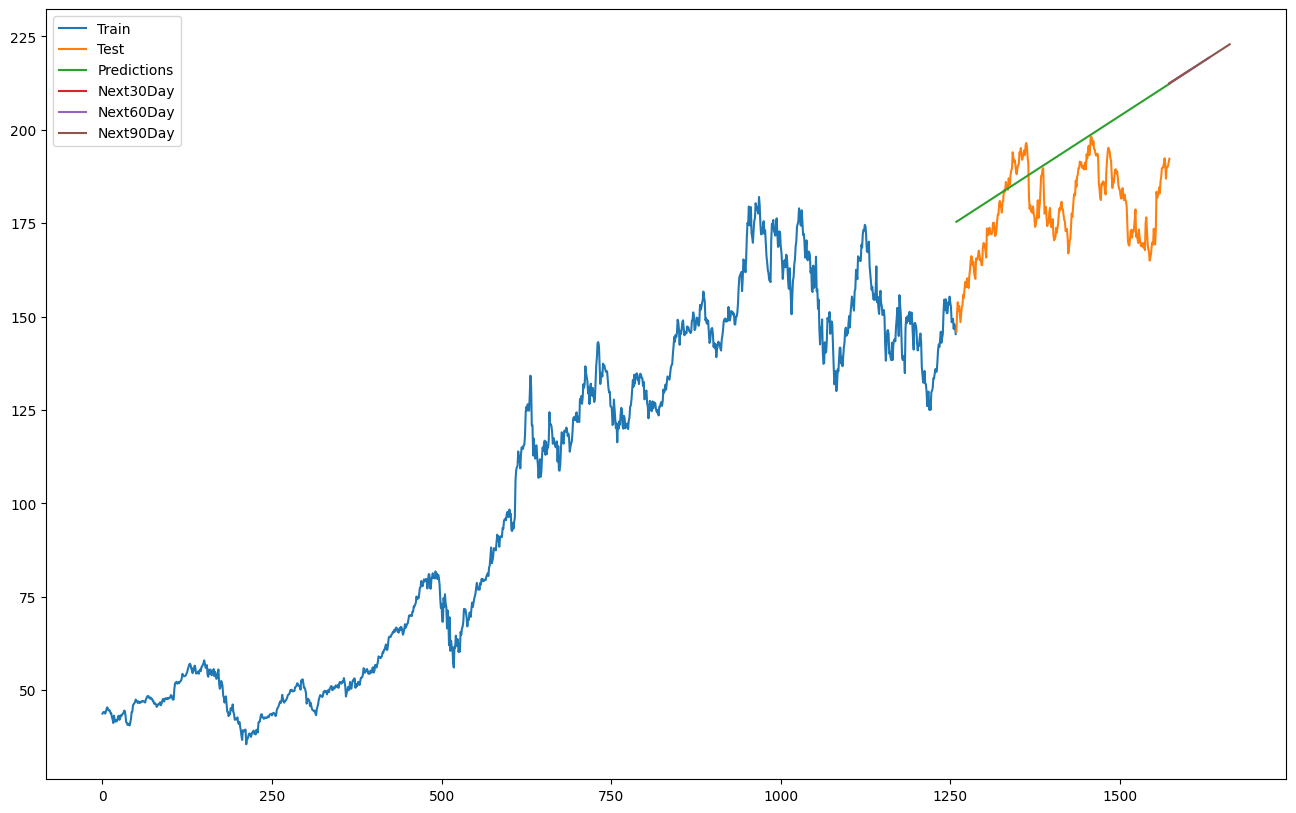
\includegraphics[width=\linewidth]{template/bibliography/Figure/LR_AAPL_8-2.png}
    \caption{Linear model's result with 8:2 splitting proportion}
    \label{fig8}
  \end{minipage}
\end{figure}

\begin{figure}[H]
  \centering
  \begin{minipage}{0.8\linewidth}
    \centering
    \includegraphics[width=\linewidth]{template//bibliography//Figure//GARCH_UPDATE/GARCH_AAPL_91.png}
    \caption{Garch model's result with 9:1 splitting proportion}
    \label{fig9}
  \end{minipage}
\end{figure}

\begin{figure}[H]
  \centering
  \begin{minipage}{0.8\linewidth}
    \centering
    \includegraphics[width=\linewidth]{template/bibliography/Figure/GRU/GRU_AAPL_91.png}
    \caption{GRU model's result with 9:1 splitting proportion}
    \label{fig13}
  \end{minipage}
\end{figure}

\begin{figure}[H]
  \centering
  \begin{minipage}{0.8\linewidth}
    \centering
    \includegraphics[width=\linewidth]{}
\begin{figure}
        \centering
        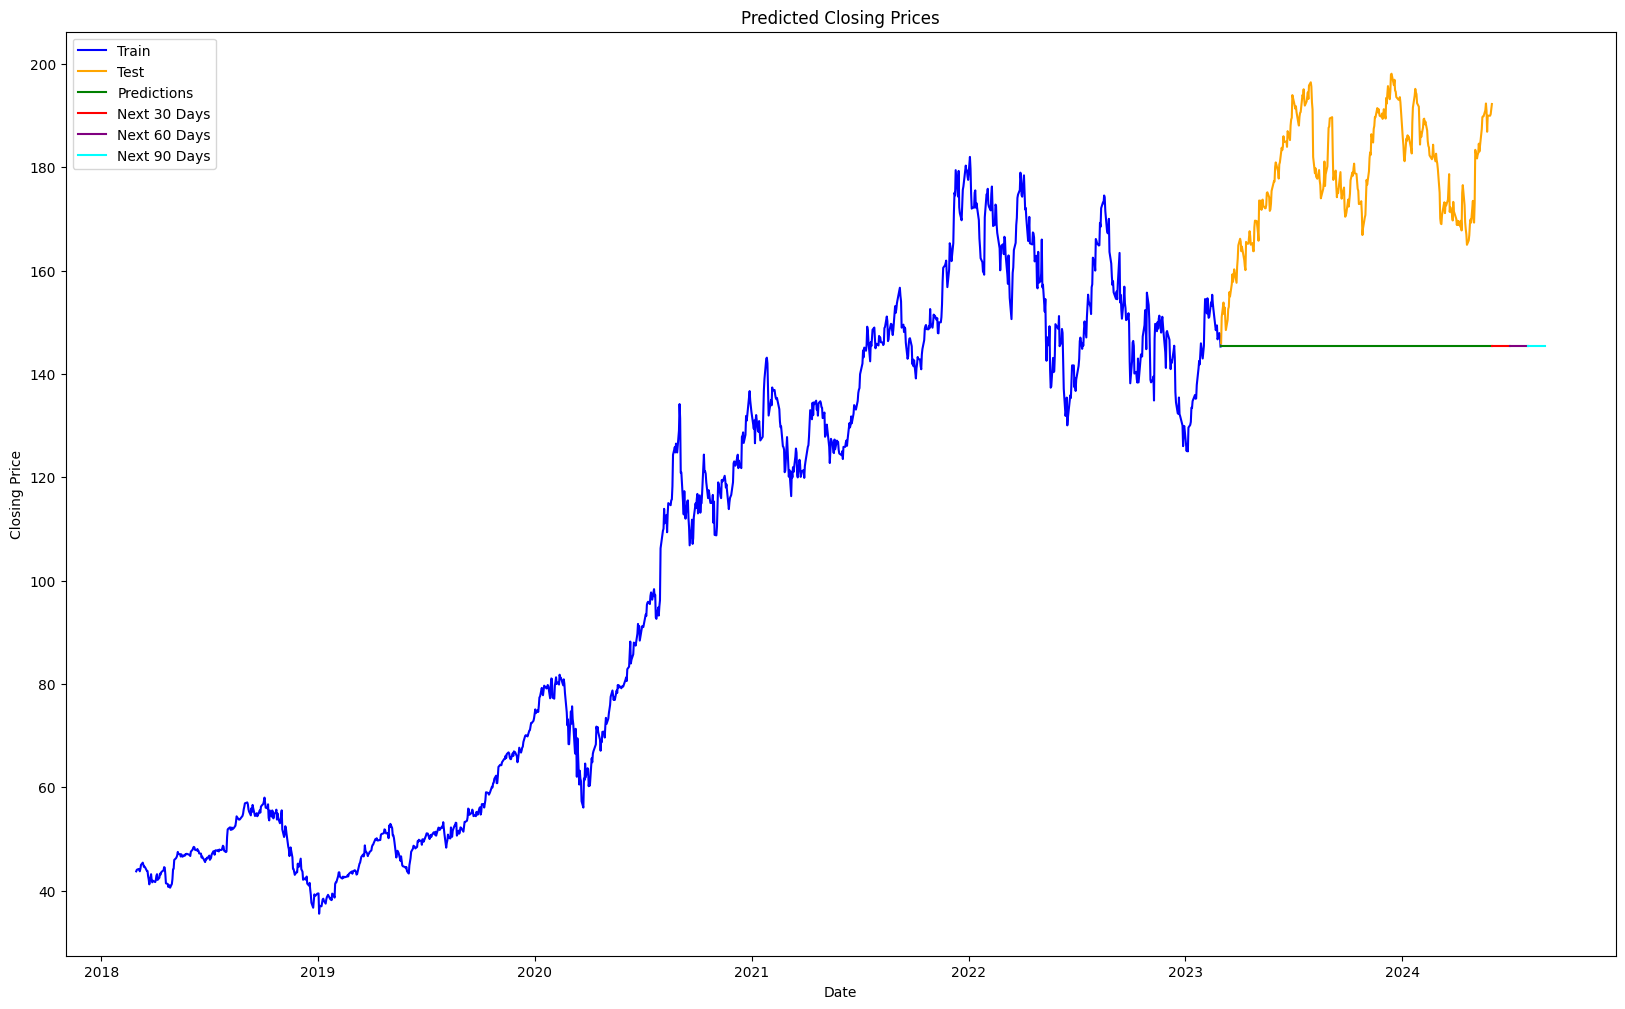
\includegraphics[width=\linewidth]{template/ARIMA AAPL 8-2.png}
        \caption{ARIMA model's result with 8:2 splitting proportion}
        \label{fig:enter-label}
    \end{figure}
    \label{fig11}
  \end{minipage}
\end{figure}
\begin{figure}[H]
  \centering
  \begin{minipage}{0.8\linewidth}
    \centering
    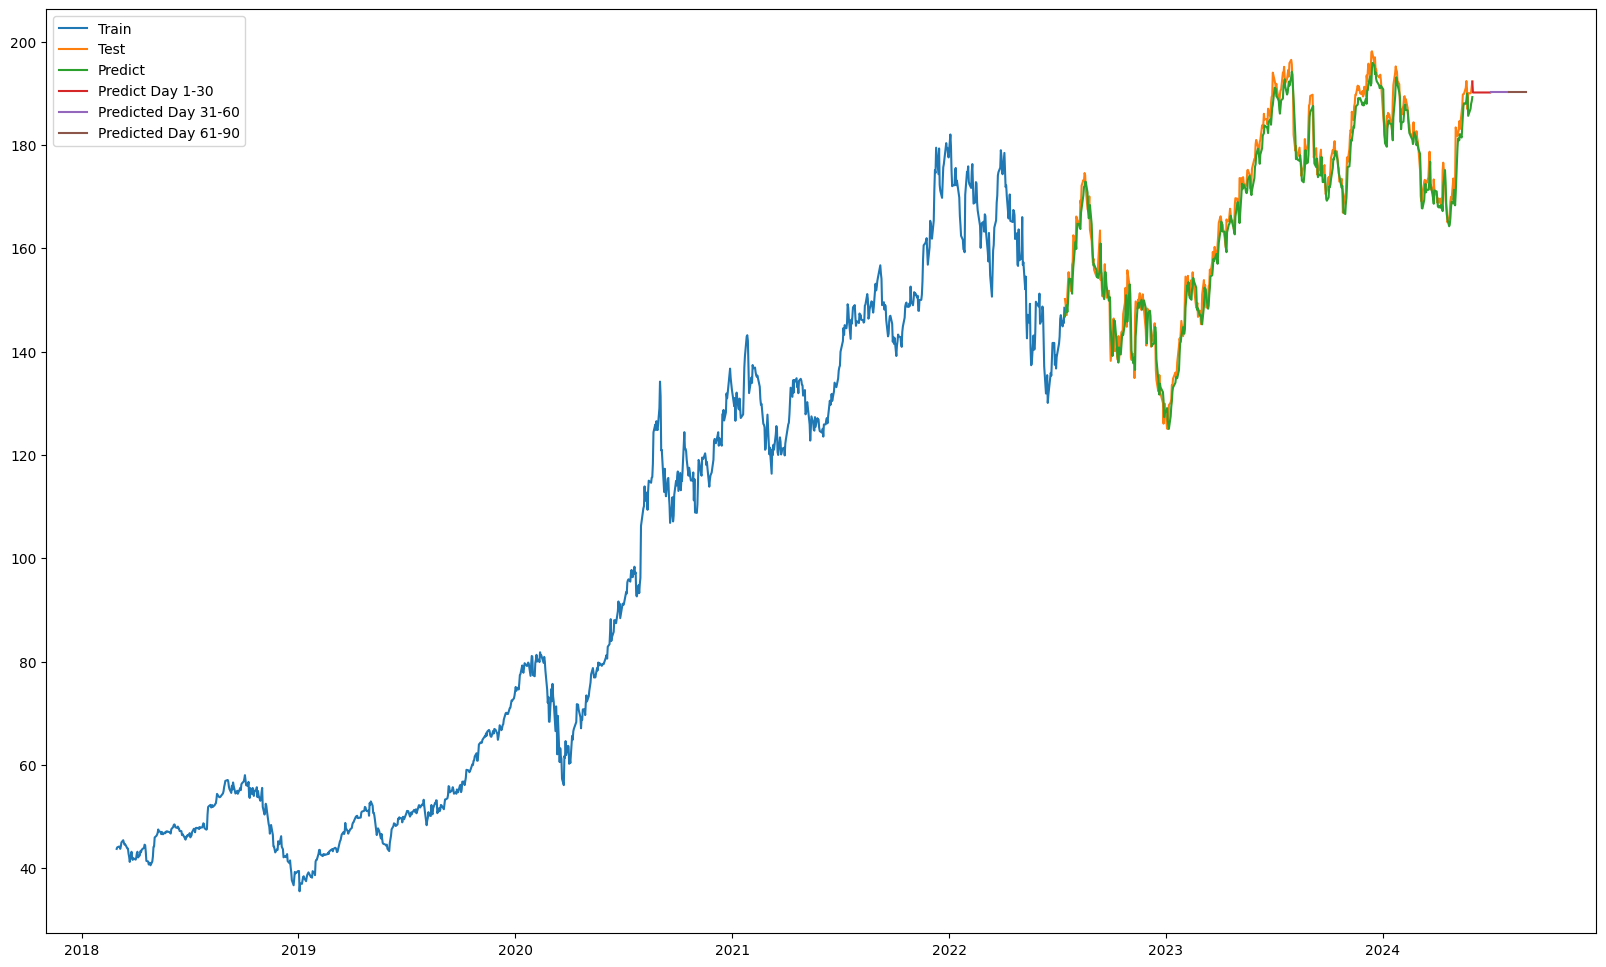
\includegraphics[width=\linewidth]{template/LSTM AAPL 7-3.png}
    \caption{LSTM model's result with 7:3 splitting proportion}
    \label{fig12}
  \end{minipage}
\end{figure}
\begin{figure}[H]
  \centering
  \begin{minipage}{0.8\linewidth}
    \centering
    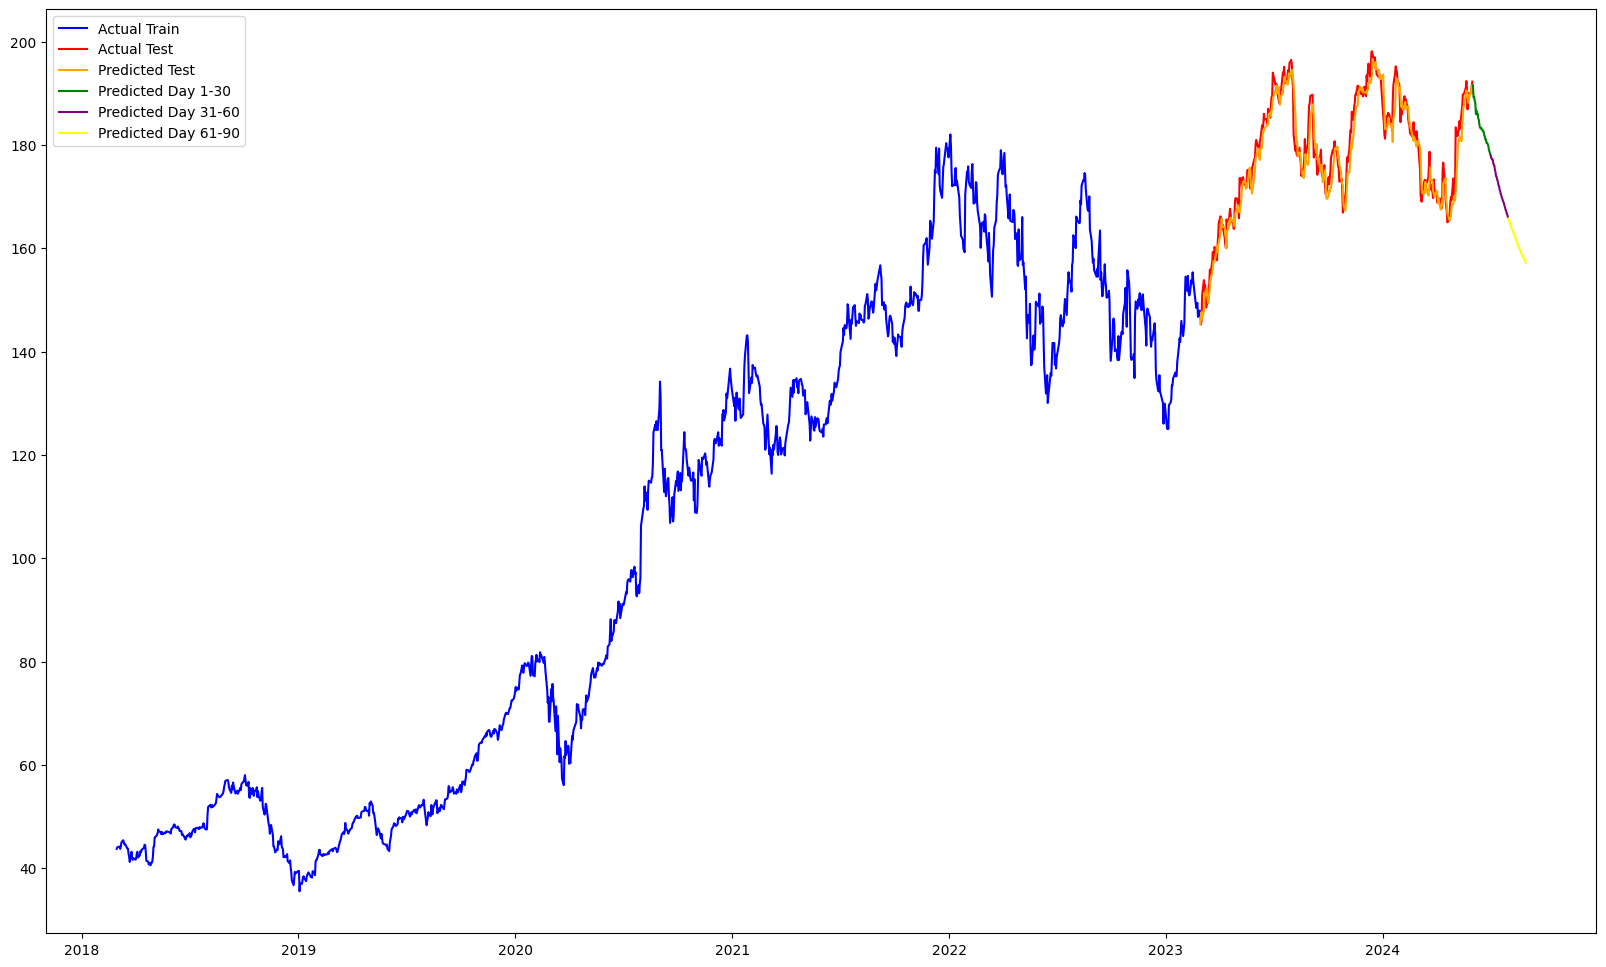
\includegraphics[width=\linewidth]{template/MLP AAPL 8-2.png}
    \caption{MLP model's result with 8:2 splitting proportion}
    \label{fig13}
  \end{minipage}
\end{figure}
\begin{figure}[H]
  \centering
  \begin{minipage}{0.8\linewidth}
    \centering
    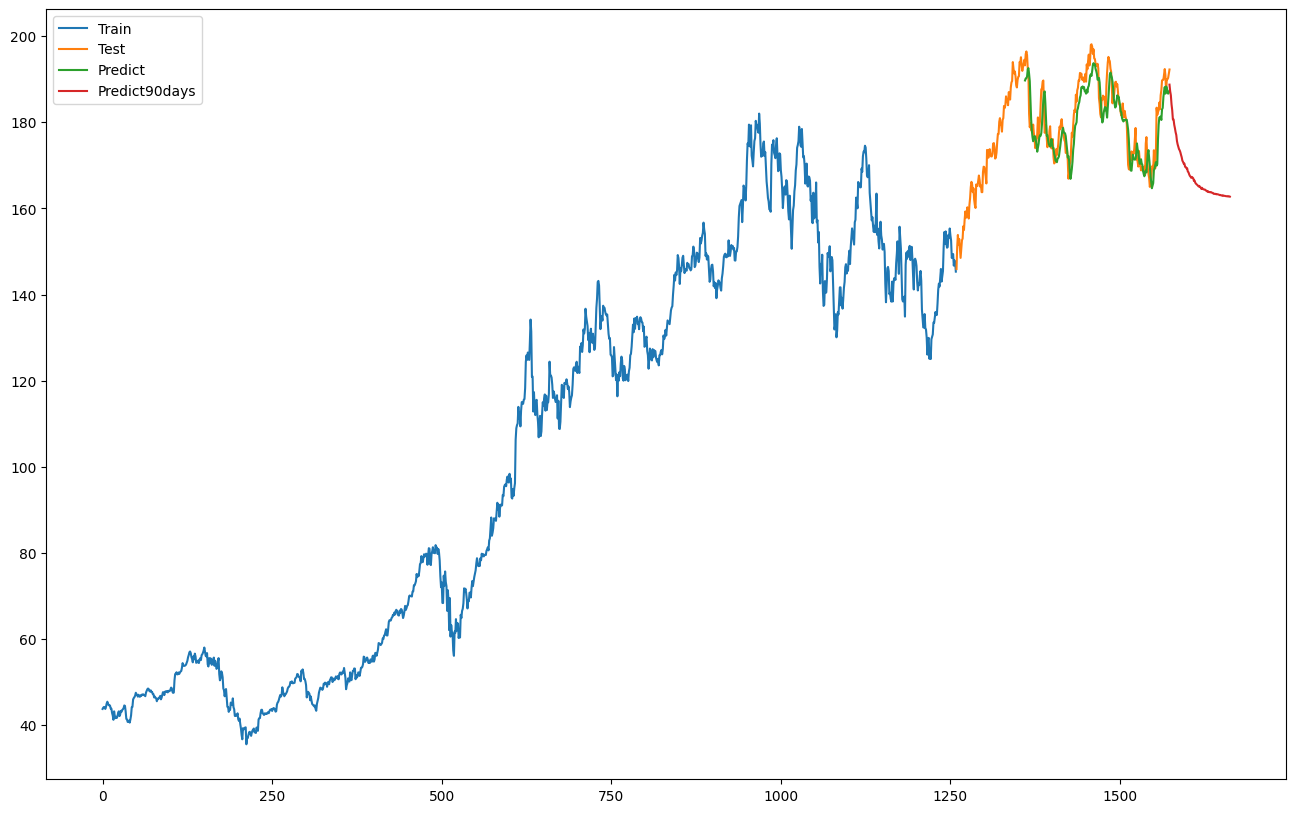
\includegraphics[width=\linewidth]{template/bibliography/Figure/RNN_AAPL_8-2.png}
    \caption{RNN model's result with 8:2 splitting proportion}
    \label{fig14}
  \end{minipage}
\end{figure}
\begin{figure}[H]
  \centering
  \begin{minipage}{0.8\linewidth}
    \centering
    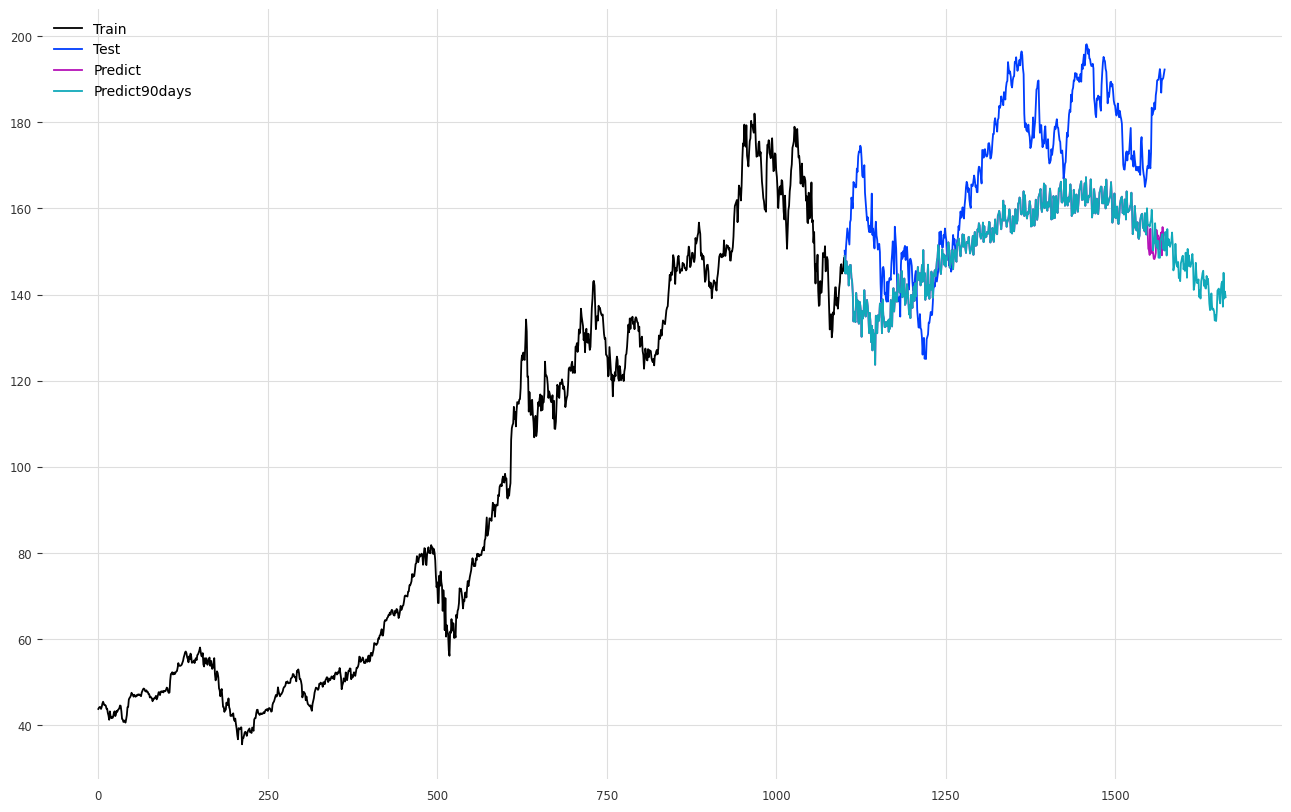
\includegraphics[width=\linewidth]{template/bibliography/Figure/TiDE/TiDE_AAPL_7-3.png}
    \caption{TiDE model's result with 7:3 splitting proportion}
    \label{bagginggru}
  \end{minipage}
\end{figure}
\subsection{MSFT Stock dataset} 
\begin{table}[H]
    \centering
    \begin{tabular}{|c|c|c|c|c|}
         \hline
         \multicolumn{5}{|c|}{\textbf{MSFT Stock Dataset's Evaluation}}\\
         \hline
         \centering Model & Training:Testing & RMSE & MAPE (\%) & MAE\\
         \hline
         \multirow{2}{*}{LR} & 7:3&61.02&18.65&51.03 
         \\ & \textbf{8:2} &  \textbf{34.57} & \textbf{7.96} & \textbf{28.71} 
         \\ & 9:1 & 47.52 & 10.83 & 43.71\\
       \hline
         \multirow{2}{*}{GARCH} & 7:3&11.235&46.99&9.312\\ & 8:2&7.808&43.18&6.495\\ & \textbf{9:1}& \textbf{5.569}& \textbf{41.434}& \textbf{4.839}\\
         \hline
         \multirow{2}{*}{GRU} & 7:3&7.111&1.735&5.646\\ &  \textbf{8:2}&\textbf{6.638}&\textbf{1.417}&	\textbf{5.247}\\ & 9:1& 6.944& 1.265& 5.211\\
         \hline
         \multirow{2}{*}{ARIMA} & 7:3 & 54.538 & 12.988 & 44.736 \\ & 8:2 & 117.390 & 29.029 & 107.4226 \\ & \textbf{9:1} & \textbf{11.885} & \textbf{5.419} & \textbf{9.629}\\
         \hline
         \multirow{2}{*}{LSTM} & 7:3 &5.805& 1.474& 4.608 \\ &\textbf{8:2} & \textbf{4.911} & \textbf{1.096} & \textbf{3.822} \\ &  9:1 &  5.700 &  1.193 &  4.697\\
         \hline
         \multirow{2}{*}{MLP} & 7:3 & 8.290 & 2.209 & 6.656 \\ & 8:2 & 6.075 & 1.379 & 4.855\\ & \textbf{9:1} & \textbf{5.728} & \textbf{1.120} & \textbf{4.408}\\
         \hline
         \multirow{2}{*}{RNN} & \textbf{7:3} &  \textbf{6.292} & \textbf{1.521} & \textbf{5.107} 
         \\ & 8:2 & 13.278 & 3.176 & 12.093
         \\ & 9:1 & 15.062 & 3.294 & 13.804 \\
         \hline
         \multirow{2}{*}{TiDE} & \textbf{7:3} & \textbf{74.635} &  \textbf{15.772} &  \textbf{54.885} 
         \\ & 8:2 & 75.311 &  14.130 &  55.084
         \\ & 9:1 & 127.371 & 29.642 & 119.175\\
         \hline
    \end{tabular}
    \caption{MSFT Stock Dataset's Evaluation}
    \label{mbbresult}
\end{table}

\begin{figure}[H]
  \centering
  \begin{minipage}{0.8\linewidth}
    \centering
    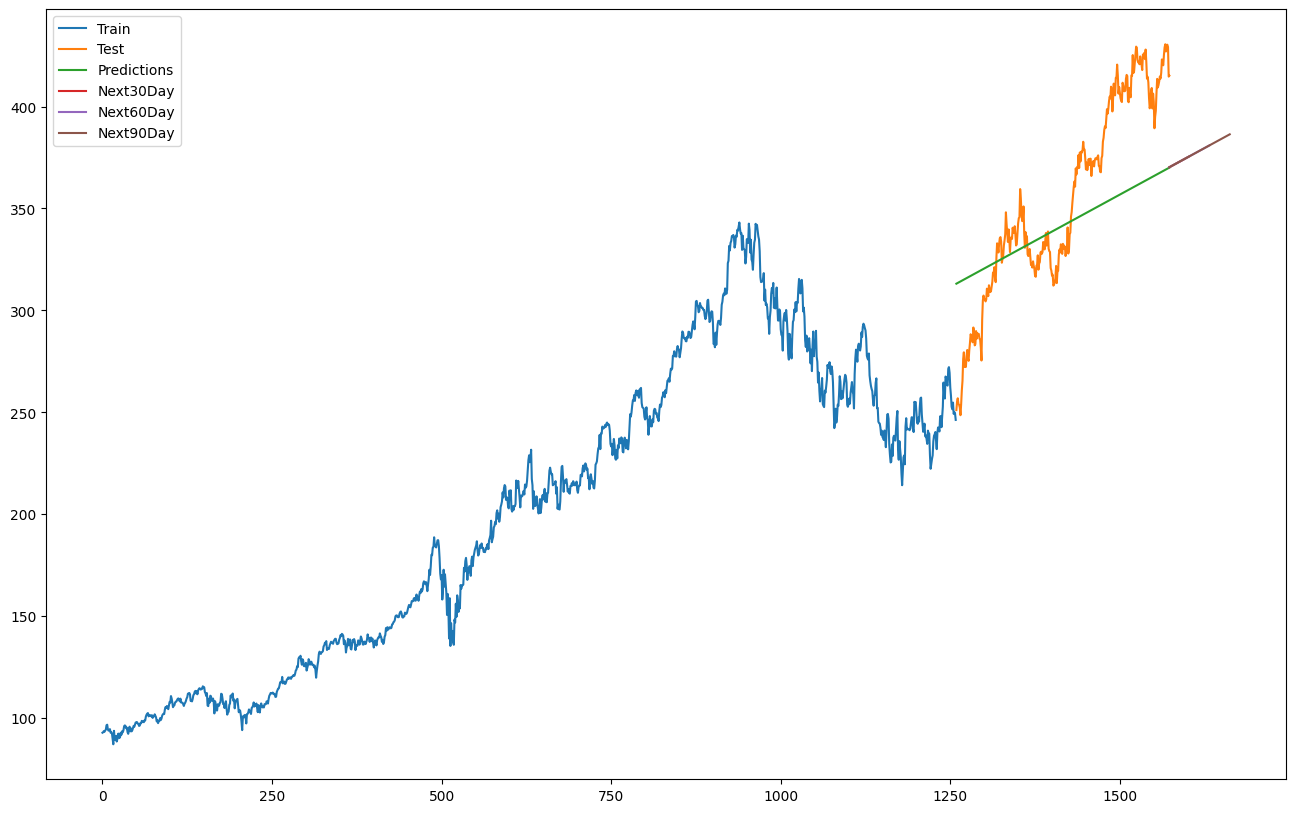
\includegraphics[width=\linewidth]{template/bibliography/Figure/LR_MSFT_8-2.png}
    \caption{Linear model's result with 8:2 splitting proportion}
    \label{fig15}
  \end{minipage}
\end{figure}
\begin{figure}[H]
  \centering
  \begin{minipage}{0.8\linewidth}
    \centering
    \includegraphics[width=\linewidth]{template/bibliography/Figure/GARCH_UPDATE/GARCH_MSFT_91.png}
    \caption{GARCH model's result with 9:1 splitting proportion}
    \label{fig16}
  \end{minipage}
\end{figure}
\begin{figure}[H]
  \centering
  \begin{minipage}{0.8\linewidth}
    \centering
    \includegraphics[width=\linewidth]{template/bibliography/Figure/GRU/GRU_MSFT_82.png}
    \caption{GRU model's result with 8:2 splitting proportion}
    \label{fig17}
  \end{minipage}
\end{figure}
\begin{figure}[H]
  \centering
  \begin{minipage}{0.8\linewidth}
    \centering
    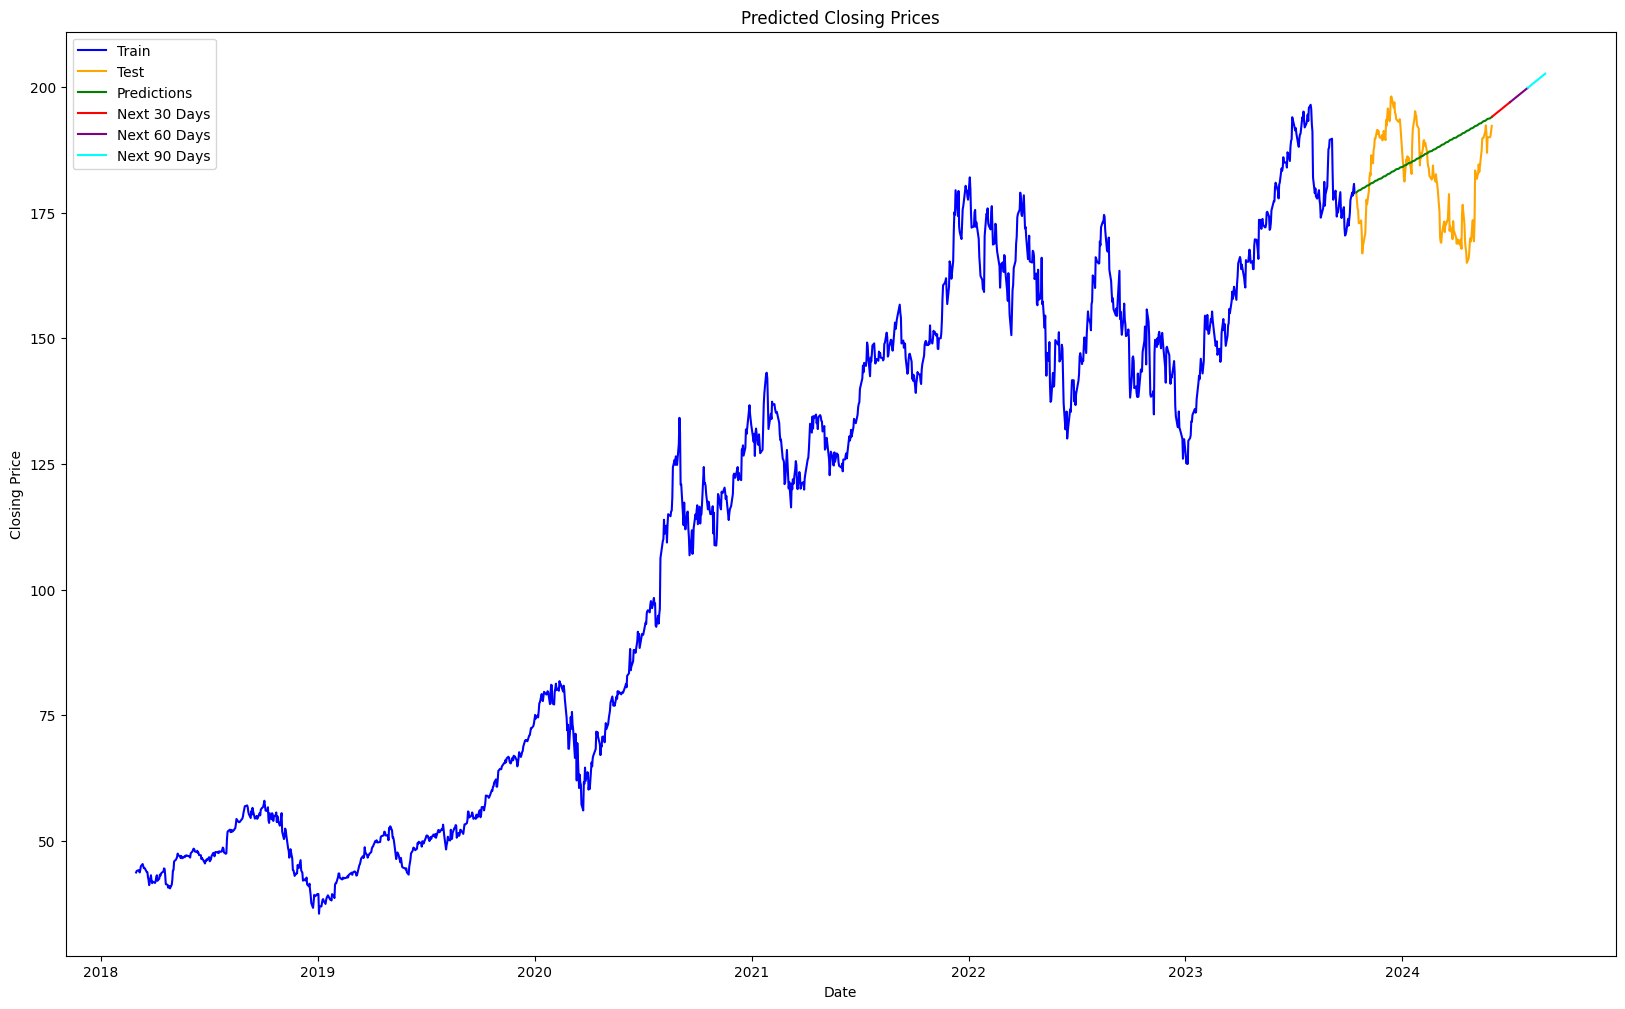
\includegraphics[width=\linewidth]{template/ARIMA MSFT 9-1.png}
    \caption{ARIMA model's result with 9:1 splitting proportion}
    \label{fig18}
  \end{minipage}
\end{figure}
\begin{figure}[H]
  \centering
  \begin{minipage}{0.8\linewidth}
    \centering
    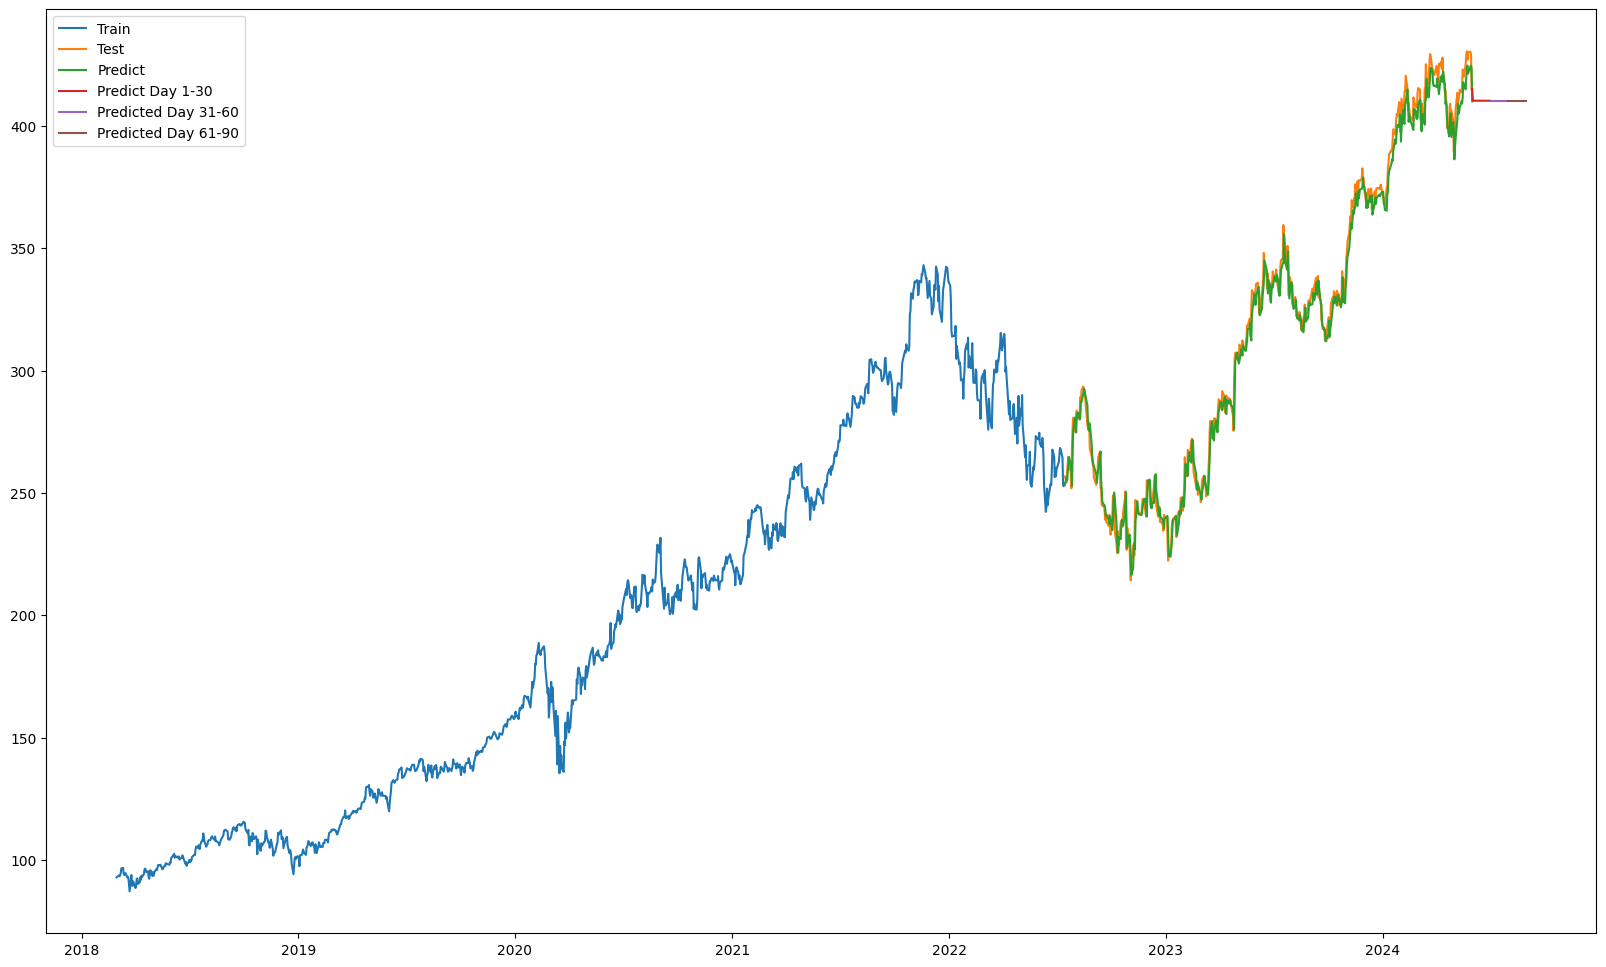
\includegraphics[width=\linewidth]{template/LSTM MSFT 7-3.png}
    \caption{LSTM model's result with 7:3 splitting proportion}
    \label{fig19}
  \end{minipage}
\end{figure}
\begin{figure}[H]
  \centering
  \begin{minipage}{0.8\linewidth}
    \centering
    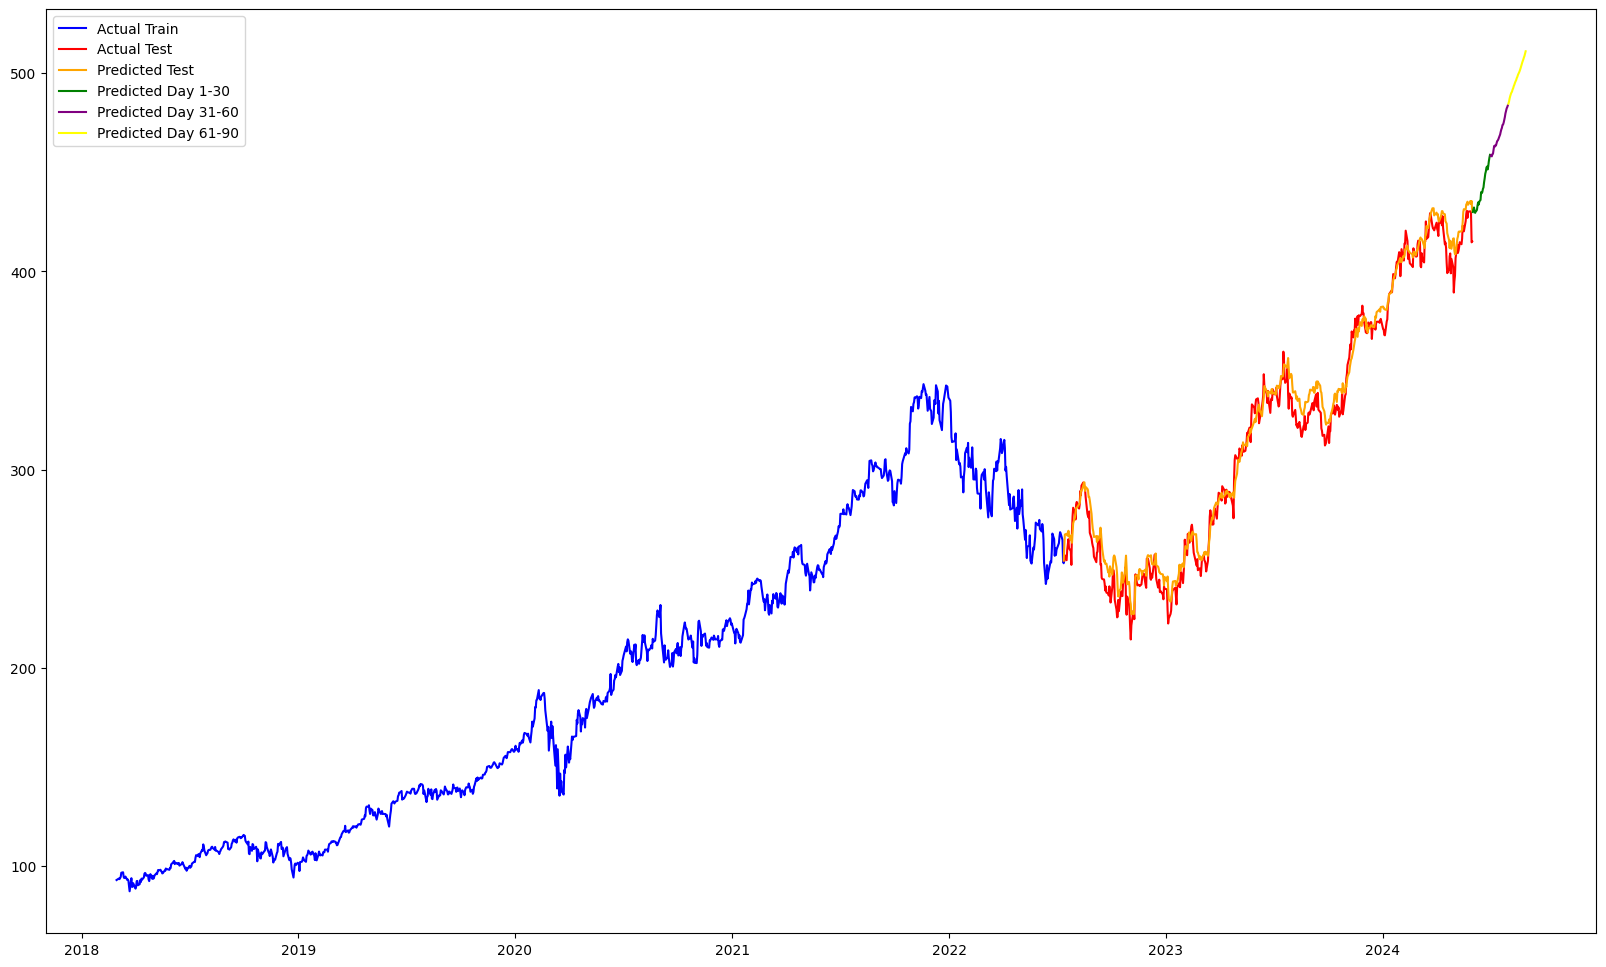
\includegraphics[width=\linewidth]{template/MLP MSFT 7-3.png}
    \caption{MLP model's result with 7:3 splitting proportion}
    \label{fig20}
  \end{minipage}
\end{figure}
\begin{figure}[H]
  \centering
  \begin{minipage}{0.8\linewidth}
    \centering
    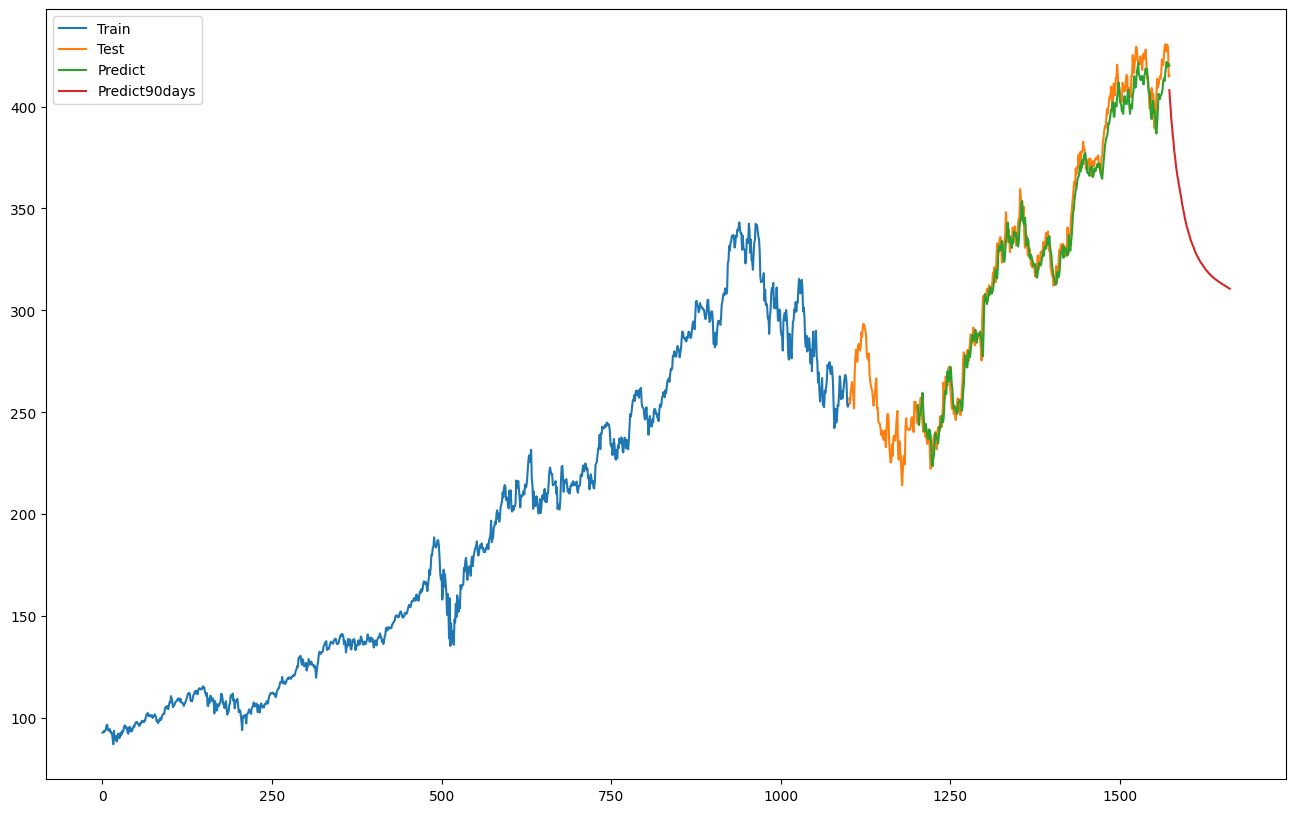
\includegraphics[width=\linewidth]{template/bibliography/Figure/RNN_MSFT_7-3.png}
    \caption{RNN model's result with 7:3 splitting proportion}
    \label{fig21}
  \end{minipage}
\end{figure}
\begin{figure}[H]
  \centering
  \begin{minipage}{0.8\linewidth}
    \centering
    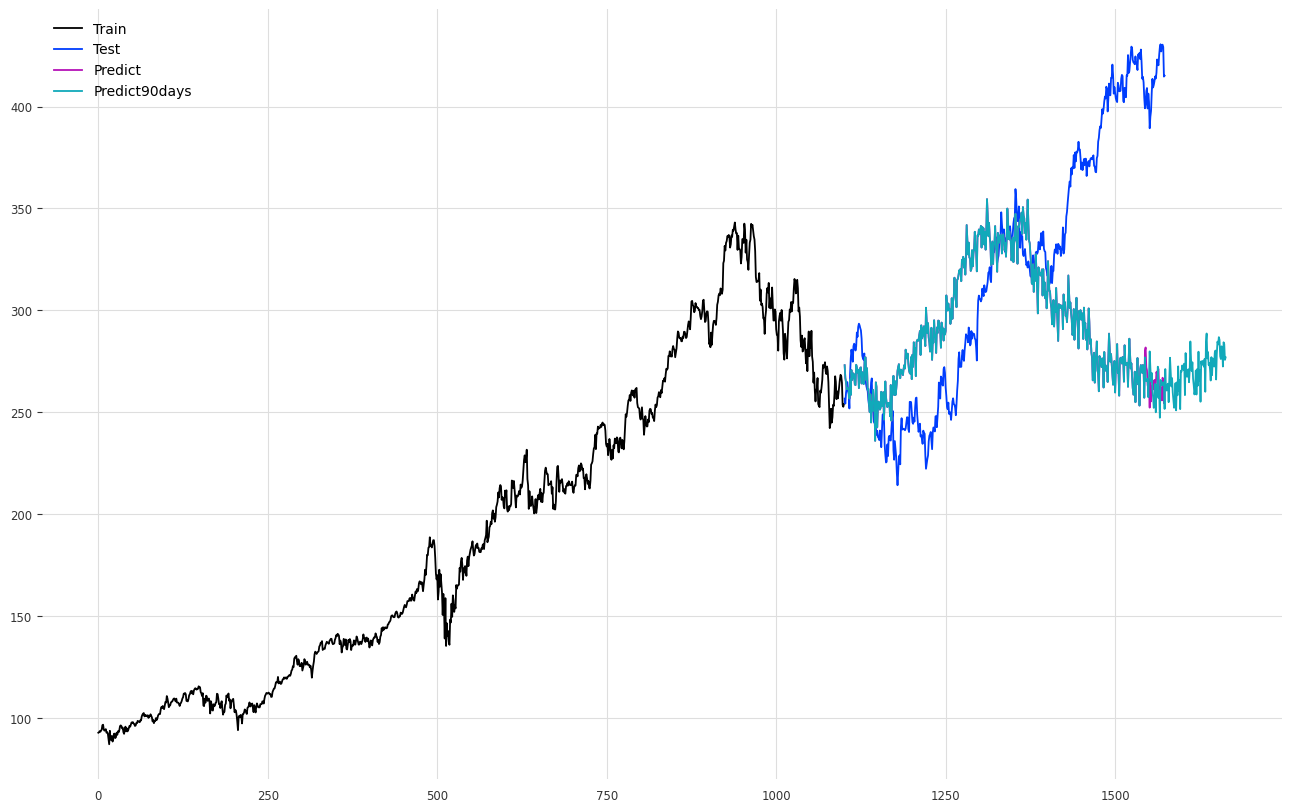
\includegraphics[width=\linewidth]{template/bibliography/Figure/TiDE/TiDE_MSFT_7-3.png}
    \caption{TiDE model's result with 7:3 splitting proportion}
    \label{mbbbggg}
  \end{minipage}
\end{figure}
\subsection{GOOG Stock dataset} 
\begin{table}[H]
    \centering
    \begin{tabular}{|c|c|c|c|c|}
         \hline
         \multicolumn{5}{|c|}{\textbf{GOOG Stock Dataset's Evaluation}}\\
         \hline
         \centering Model & Training:Testing & RMSE & MAPE (\%) & MAE\\
         \hline
         \multirow{2}{*}{LR} & 7:3&36.39&30.33&33.86 \\ & 8:2 &  15.25 & 9.82 & 12.01 \\ & \textbf{9:1}&\textbf{13.53}&\textbf{6.20}&\textbf{9.76}\\
      \hline
         \multirow{2}{*}{GARCH} & 7:3&16.158&46.673&
13.691\\ & 8:2&12.666&40.463&10.831\\ & \textbf{9:1} & \textbf{13.320}& \textbf{38.568}& \textbf{10.831}\\
         \hline
         \multirow{2}{*}{GRU} & 7:3 & 3.463& 2.131& 2.630\\ &  8:2 & 3.410& 1.811& 2.564\\ & \textbf{9:1} &\textbf{3.392}& \textbf{1.608}& \textbf{2.566}\\
         \hline
         \multirow{2}{*}{ARIMA} & 7:3 & 25.446 & 16.146 & 20.922 \\ & 8:2 & 47.351 & 30.924 & 43.353 \\ & \textbf{9:1} & \textbf{12.202} & \textbf{5.727} & \textbf{8.884}\\
         \hline
         \multirow{2}{*}{LSTM} & \textbf{7:3} & \textbf{2.678} & \textbf{1.642} & \textbf{1.987} \\ &8:2 &2.763 & 1.500 & 1.980 \\ &  9:1 & 2.847& 1.257 & 1.849\\
         \hline
         \multirow{2}{*}{MLP} & 7:3 & 4.720 & 3.294 & 3.869\\ & 8:2 & 5.006	& 3.056 & 4.226\\ &\textbf{ 9:1 }& \textbf{3.551} & \textbf{1.855} & \textbf{2.742}\\
         \hline
         \multirow{2}{*}{RNN} & 7:3 & 2.776 & 1.668 & 2.080 
         \\ & \textbf{8:2} & \textbf{2.886} & \textbf{1.450} & \textbf{2.103} 
         \\ & 9:1 & 3.678 &	1.744 & 2.836 \\
         \hline
         \multirow{2}{*}{TiDE} & \textbf{7:3} & \textbf{16.034} &  \textbf{9.718} &  \textbf{11.815} 
         \\ & 8:2 & 40.055 & 28.255 & 38.367 
         \\ & 9:1 & 23.957 & 10.385 & 16.536\\
         \hline
    \end{tabular}
    \caption{GOOG Stock Dataset's Evaluation}
    \label{mbbresult}
\end{table}

\begin{figure}[H]
  \centering
  \begin{minipage}{0.8\linewidth}
    \centering
    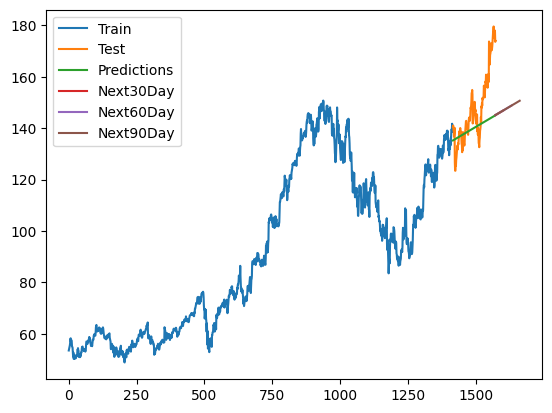
\includegraphics[width=\linewidth]{template/bibliography/Figure/LR_GOOG_9-1.png}
    \caption{Linear model's result with 9:1 splitting proportion}
    \label{fig22}
  \end{minipage}
\end{figure}
\begin{figure}[H]
  \centering
  \begin{minipage}{0.8\linewidth}
    \centering
    \includegraphics[width=\linewidth]{template//bibliography//Figure//GARCH_UPDATE/GARCH_GOOG_91.png}
    \caption{GARCH model's result with 9:1 splitting proportion}
    \label{fig23}
  \end{minipage}
\end{figure}
\begin{figure}[H]
  \centering
  \begin{minipage}{0.8\linewidth}
    \centering
    \includegraphics[width=\linewidth]{template/bibliography/Figure/GRU/GRU_GOOG_91.png}
    \caption{GRU model's result with 9:1 splitting proportion}
    \label{fig24}
  \end{minipage}
\end{figure}
\begin{figure}[H]
  \centering
  \begin{minipage}{0.8\linewidth}
    \centering
    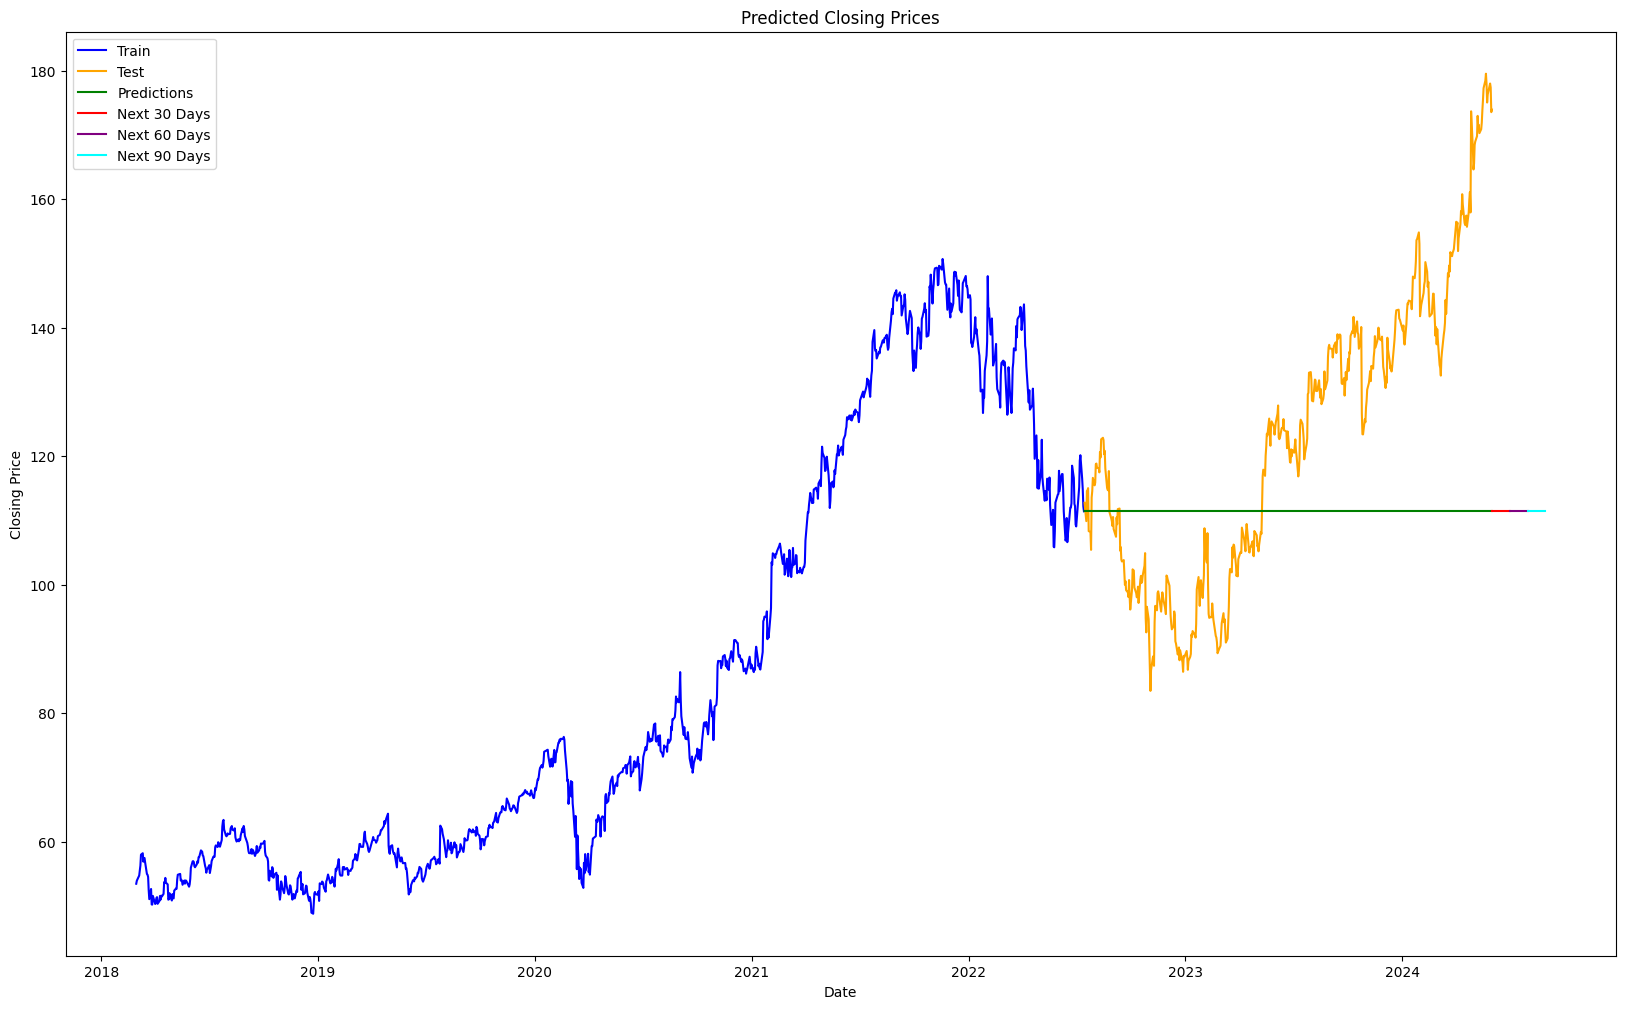
\includegraphics[width=\linewidth]{template/ARIMA GOOG 7-3.png}
    \caption{ARIMA model's result with 7:3 splitting proportion}
    \label{fig25}
  \end{minipage}
\end{figure}
\begin{figure}[H]
  \centering
  \begin{minipage}{0.8\linewidth}
    \centering
    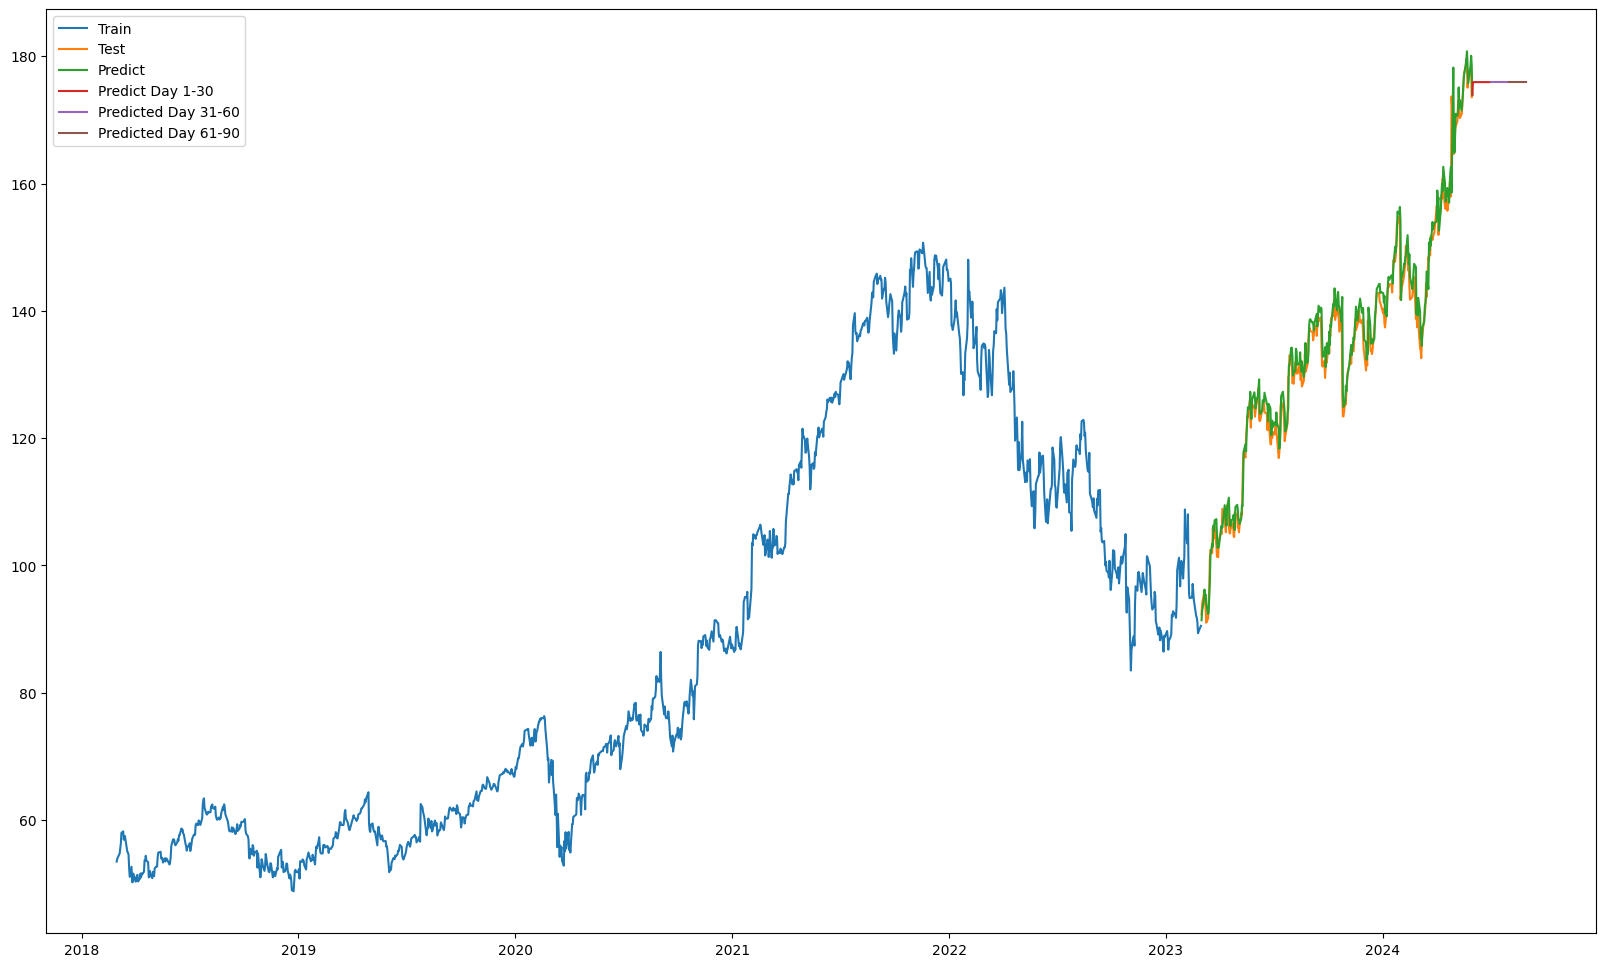
\includegraphics[width=\linewidth]{template/LSTM GOOG 8-2.png}
    \caption{LSTM model's result with 8:2 splitting proportion}
    \label{fig26}
  \end{minipage}
\end{figure}
\begin{figure}[H]
  \centering
  \begin{minipage}{0.8\linewidth}
    \centering
        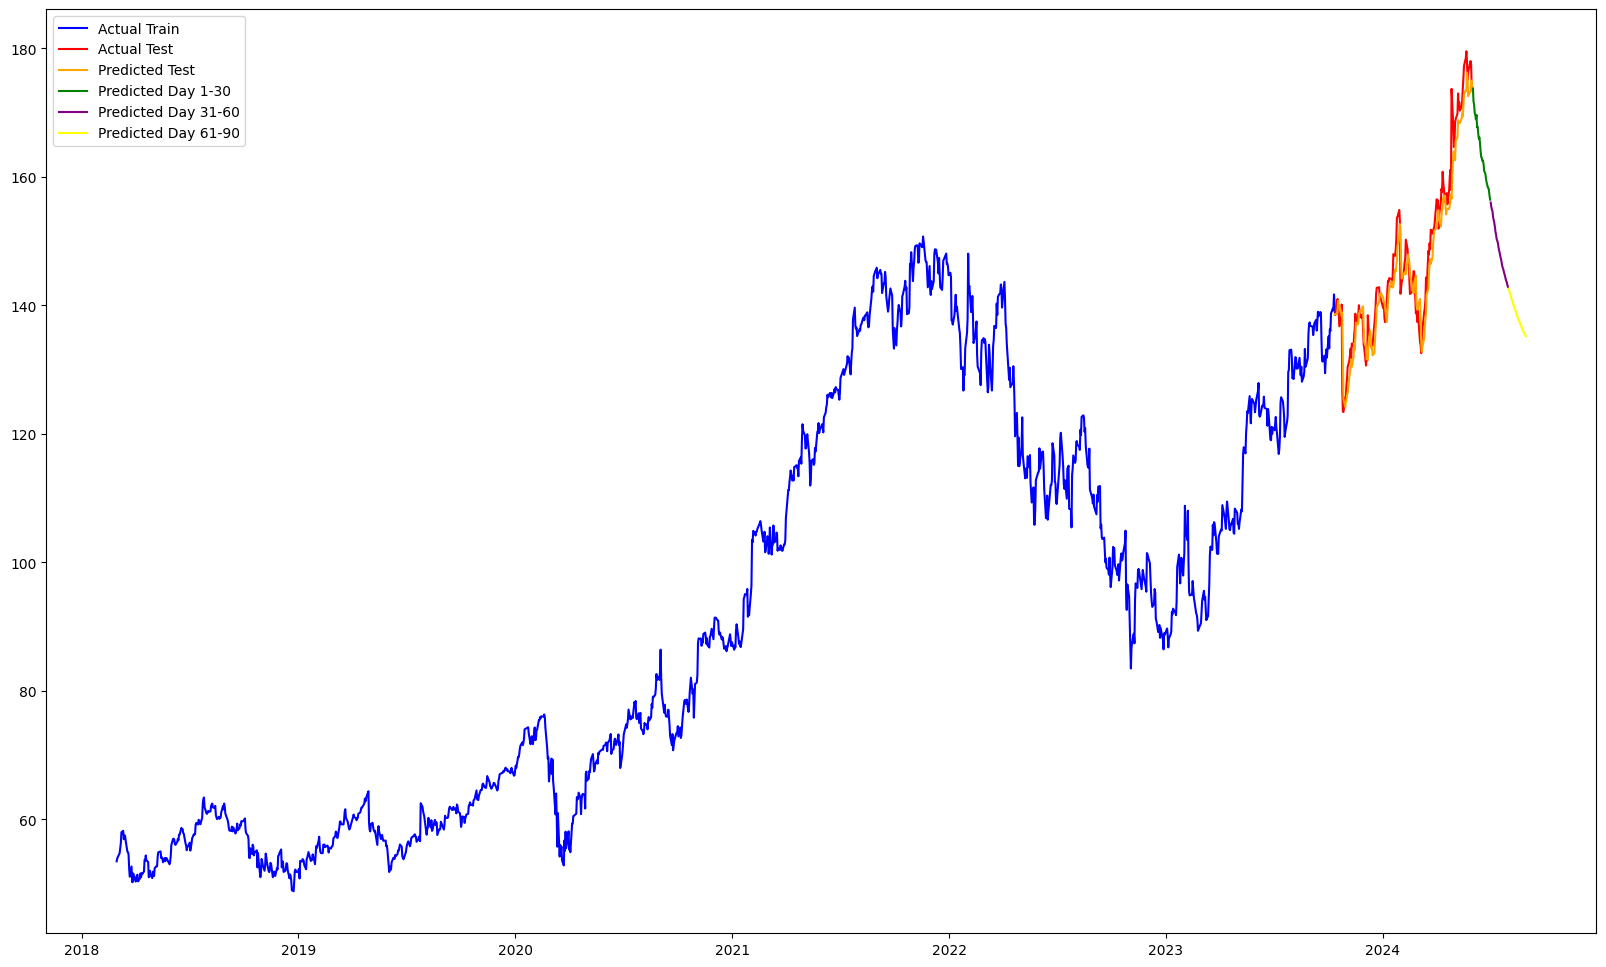
\includegraphics[width=\linewidth]{template/MLP GOOG 9-1.png}
    \caption{MLP model's result with 9:1 splitting proportion}
    \label{fig27}
  \end{minipage}
\end{figure}
\begin{figure}[H]
  \centering
  \begin{minipage}{0.8\linewidth}
    \centering
        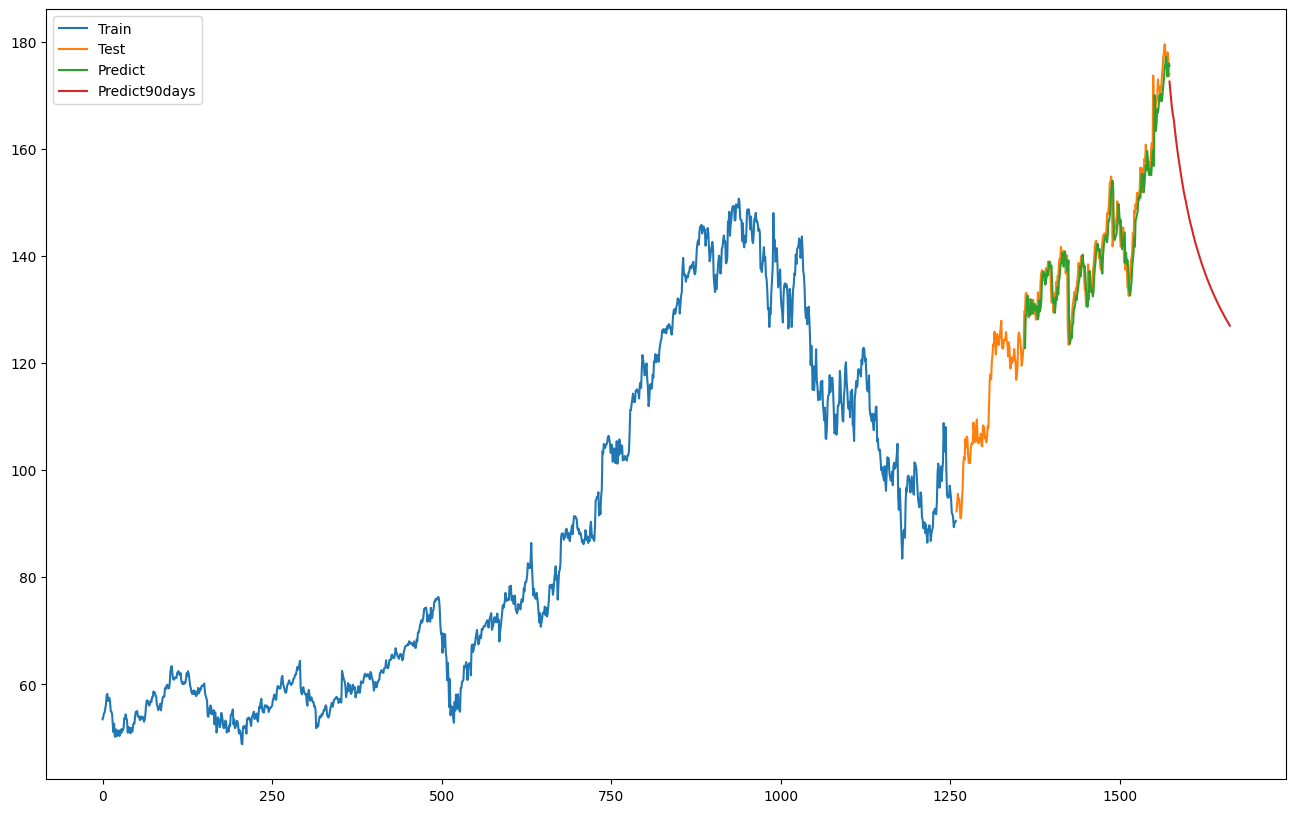
\includegraphics[width=\linewidth]{template/bibliography/Figure/RNN_GOOG_8-2.png}
    \caption{RNN model's result with 8:2 splitting proportion}
    \label{fig28}
  \end{minipage}
\end{figure}
\begin{figure}[H]
  \centering
  \begin{minipage}{0.8\linewidth}
    \centering
        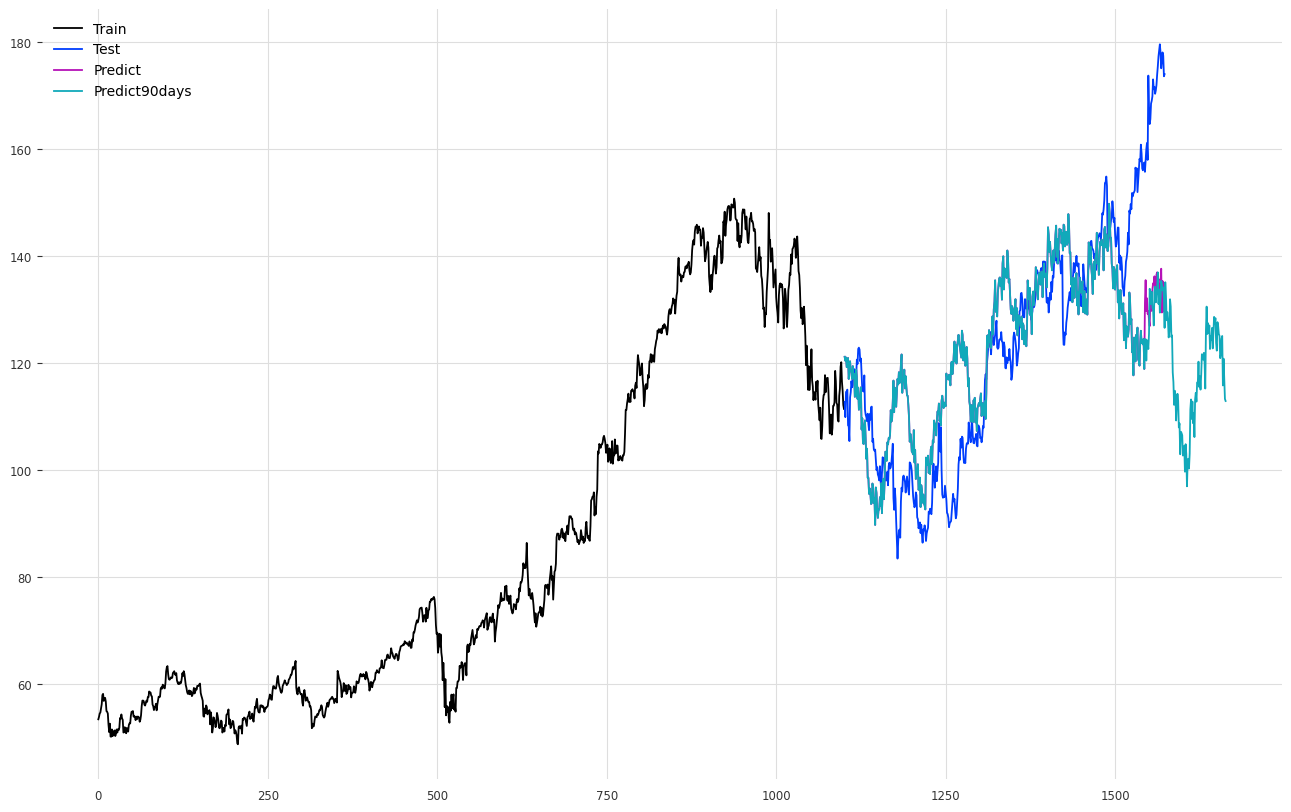
\includegraphics[width=\linewidth]{template/bibliography/Figure/TiDE/TiDE_GOOG_7-3.png}
    \caption{TiDE model's result with 7:3 splitting proportion}
    \label{fig28}
  \end{minipage}
\end{figure}



\section{Conclusion}

\subsection{Summary}
In the achievement of forecasting stock prices, the exploration of diverse methodologies, ranging from traditional statistical models to advanced machine learning algorithms, has been aimed. Among the performed models, Linear Regression, Autoregressive Integrated Moving Average (ARIMA), Long Short Term Memory (LSTM), Regression Neural Networks (RNN), Gated Regression Units (GRU), Generalized Autoregressive Conditional Heteroskedasticity (GARCH), Time-series Dense Encoder Model (TiDE), and Multi-layer Perceptron (MLP), it becomes evident that Regression Neural Networks (RNN), Long Short Term Memory (LSTM), and Multi-layer Perceptron (MLP) emerge as the most promising and effective models for predicting stock prices.\\
Regression Neural Networks (RNN), Long Short Term Memory (LSTM), and Multi-layer Perceptron (MLP) each offer distinct advantages in the realm of time-series stock price forecasting. RNNs are particularly adept at capturing and modeling sequential dependencies within time-series data, making them well-suited for financial markets where past prices influence future trends. LSTMs, an advanced type of RNN, excel in managing long-term dependencies and mitigating issues related to vanishing gradients, thereby providing more accurate and stable predictions over longer periods. MLPs, while simpler, are highly effective in capturing nonlinear relationships within the data, offering flexibility and robust performance across various market conditions. Collectively, these models leverage their unique strengths to deliver superior forecasting accuracy, adaptability to volatile market dynamics, and valuable insights for investors and analysts.\\
As evidenced by the evaluation metrics, including RMSE, MAPE, and MAE, the RNN, LSTM, and MLP models consistently demonstrate superior performance across various aspects of forecasting accuracy. Their adaptability to handle the inherent uncertainties of stock markets positions them as formidable tools for investors and analysts seeking reliable predictions.
\subsection{Future Considerations}
In our future research, it is crucial to prioritize further optimization of the previously mentioned models. This optimization effort should specifically focus on:\\
\indent\textbullet\ Enhancing the accuracy of the model. While the above algorithms have demonstrated promising results in predicting stock prices, there is a need to further improve the model's accuracy to ensure more precise forecasting outcomes.\\
\indent\textbullet\ Exploring alternative machine learning algorithms or ensemble techniques. Ensemble techniques, such as combining multiple models or using various ensemble learning methods, can also improve the robustness and accuracy of the forecasts.\\
\indent\textbullet\ Researching new forecasting models. The field of forecasting continuously evolves, with new algorithms and models being researched and developed. It is crucial to stay updated with these approaches and explore new forecasting models that offer improved accuracy and performance. \\
By continuously exploring and incorporating new features, data sources, and modeling techniques, we can strive for ongoing optimization of the forecasting models and enhance their ability to predict stock prices with greater precision and reliability.
\section*{Acknowledgment}
\addcontentsline{toc}{section}{Acknowledgment}
First and foremost, we would like to express our sincere gratitude to \textbf{Assoc. Prof. Dr. Nguyen Dinh Thuan} and \textbf{Mr. Nguyen Minh Nhut} for their exceptional guidance, expertise, and invaluable feedback throughout the research process. Their mentorship and unwavering support have been instrumental in shaping the direction and quality of this study. Their profound knowledge, critical insights, and attention to detail have significantly contributed to the success of this research.
\\This research would not have been possible without the support and contributions of our mentors. We would like to extend our heartfelt thanks to everyone involved for their invaluable assistance, encouragement, and belief in our research. Thank you all for your invaluable assistance and encouragement.
# 
\begin{thebibliography}{00}

\bibitem{b1} L. Li, Y. Yabin, Y. Ou, Q. Li, Y. Zhou, and D. Chen, "Research on machine learning algorithms and feature extraction for time series." In \textit{Proceedings of the International Conference on Machine Learning and Cybernetics}, 2018, pp. 123-128.

\bibitem{b2} S. Hochreiter and J. Schmidhuber, “Long Short-Term Memory,” \textit{Neural Computation}, vol. 9, no. 8, pp. 1735–1780, Nov. 1997, doi: 10.1162/neco.1997.9.8.1735.

\bibitem{b3} S. S. Namin and A. S. Namin, “Forecasting Economic Variables with Long Short Term Memory (LSTM) Neural Networks," in \textit{2018 17th IEEE International Conference on Machine Learning and Applications (ICMLA)}, 2018, pp. 1241-1246, doi: 10.1109/ICMLA.2018.00203.

\bibitem{b4} N. T. Hien, "Application of ARCH-GARCH model to analyze the fluctuation of VNIndex," \textit{Journal of Science and Technology}, vol. 126, no. 1MEIS, pp. 18-25, 2019. [Online]. Available: https://tckhtm.tmu.edu.vn/upload/news/files/126-b2.pdf

\bibitem{b5} X. Jiang, “Bitcoin Price Prediction Based on Deep Learning Methods,” \textit{Journal of Mathematical Finance}, vol. 10, no. 2, pp. 252-263, 2020. [Online]. Available: https://www.scirp.org/pdf/jmf\_2020021013592656.pdf

\bibitem{b6} D. Bhuriya, G. Kaushal, A. Sharma, and U. Singh, "Stock market prediction using a linear regression," in \textit{2017 International Conference of Electronics, Communication and Aerospace Technology (ICECA)}, vol. 2, 2017, pp. 510-513. doi: 10.1109/ICECA.2017.8203539.

\bibitem{b7} Y. Zhu, "Stock price prediction using the RNN model," in \textit{2020 International Conference on Applied Physics and Computing (ICAPC 2020)}, 2020. doi: 10.1088/1742-6596/1650/3/032103.

\bibitem{b8} Long Short Term Memory Cell. \textit{Designs}, vol. 14, no. 11, p. 1696, Nov. 2023. [Online]. Available: https://www.mdpi.com/2073-4433/14/11/1696.

\bibitem{b9} A. Das, S. Ghosh, and S. Sen, "Long-term Forecasting with TIDE: Time-series Dense Encoder," arXiv preprint arXiv:2304.08424, 2023.

\bibitem{b10} R. Guedes, "TIDE: the 'embarrassingly' simple MLP that beats Transformers," \textit{Medium}, Mar. 01, 2024. [Online]. Available: https://towardsdatascience.com/tide-the-embarrassingly-simple-mlp-that-beats-transformers-7db77d588079

\bibitem{b11} "Time Series Forecasting using Recurrent Neural Networks (RNN) in TensorFlow," \textit{GeeksforGeeks}, Jul. 31, 2023. [Online]. Available: https://www.geeksforgeeks.org/time-series-forecasting-using-recurrent-neural-networks-rnn-in-tensorflow/

\end{thebibliography}

%%%%%%%%%%%%%%%

\EOD

\end{document}

